
%CLASSE-------------------------------------------------------------------

% verso e anverso:
\documentclass[12pt,
              openright,
              twoside,
              a4paper,
              english,
              french,
              spanish,
              sumario=tradicional,
              brazil
              ]{abntex2}

% apenas verso:
% \documentclass[12pt,oneside,a4paper,english,french,spanish,brazil]{abntex2}


%PACOTES------------------------------------------------------------------

% ---
% Pacotes fundamentais
% ---
\usepackage{lmodern}			  % Usa a fonte Latin Modern
\usepackage[T1]{fontenc}		% Selecao de codigos de fonte.
\usepackage[utf8]{inputenc} % Codificacao do documento
\usepackage{indentfirst}		% Indenta o primeiro parágrafo de cada seção.
\usepackage{color}				  % Controle das cores
\usepackage{graphicx}       % Inclusão de gráficos
\usepackage{microtype}      % PDF fica melhor
\usepackage{cmap}           % Mapear caracteres especiais no PDF
\usepackage{pgfplots}
% ---

% ---
% Demais pacotes
% ---
\usepackage{amsmath, amsfonts, amssymb, amsthm} % Mat. avançada
\usepackage{multirow}        % Para criar tabelas
\usepackage{array}           % Tabelas
\usepackage{caption}
\usepackage{subfig}
\usepackage[lite]{mtpro2}    % Fonte matemática melhorada
\newcolumntype{L}{>{\centering\arraybackslash}m{0.55\linewidth}}

% ---
% Pacotes de citações
% ---
\usepackage[brazilian,hyperpageref]{backref} %Páginas citadas na bibl.
\usepackage[alf]{abntex2cite}         % Citações padrão ABNT
\usepackage{lastpage}                 % Usado pela Ficha catalográfica

% ---
% CONFIGURAÇÕES DE PACOTES
% ---

% ---
% Configurações do pacote backref
% Usado sem a opção hyperpageref de backref
\renewcommand{\backrefpagesname}{Citado na(s) página(s):~}
% Texto padrão antes do número das páginas
\renewcommand{\backref}{}
% Define os textos da citação
\renewcommand*{\backrefalt}[4]{
	\ifcase #1 %
		Nenhuma citação no texto.%
	\or
		Citado na página #2.%
	\else
		Citado #1 vezes nas páginas #2.%
	\fi}%
% ---

% ---
% Configurações dos pacotes matemáticos
% Definindo um operador para o seno
\newcommand{\sen}{\operatorname{sen}}
\newtheorem{teorema}{Teorema}[section]
\graphicspath{{img/}}
\pgfplotsset{compat=newest}
\pgfplotsset{plot coordinates/math parser=false}
\addto\captionsbrazil{\renewcommand{\figurename}{Fig.}}
%\usepgfplotslibrary{external}
%\usetikzlibrary{external}
%\tikzexternalize
%\usetikzlibrary{external}
%\tikzset{external/system call={latex \tikzexternalcheckshellescape -halt-on-error -interaction=batchmode -jobname "\image" "\texsource"}}
%\tikzexternalize[shell escape=-enable-write18]
\newsavebox{\fmbox}
\newenvironment{fmpage}[1]
{\begin{lrbox}{\fmbox}\begin{minipage}{#1}}
{\end{minipage}\end{lrbox}\fbox{\usebox{\fmbox}}}
% ---

% ---
% INICIO DAS CUSTOMIZACOES PARA A UNIVERSIDADE XXX
% ---

% alterando a capa
\renewcommand{\imprimircapa}{%
  \begin{capa}%
    \center
    \ABNTEXchapterfont\bfseries{UNIVERSIDADE FEDERAL DO PAMPA}

    \vspace*{5cm}

    {\ABNTEXchapterfont\bfseries{MARCELO HAHN DURGANTE}}

    \vspace*{3cm}

    \ABNTEXchapterfont\bfseries{CONTROLE ADAPTATIVO DE CORRENTE EM CONVERSORES CONECTADOS NA REDE ELÉTRICA NUMA ESTRUTURA MULTIMALHA}
    \vfill

    \normalsize\textbf{Alegrete}

    \par

    \normalsize\textbf{2014}

    %\vspace*{1cm}
  \end{capa}
}


% folha de rosto

\makeatletter

\renewcommand{\folhaderostocontent}{
\begin{center}
{\ABNTEXchapterfont\bfseries{MARCELO HAHN DURGANTE}}

\vspace*{5cm}

\begin{center}
\ABNTEXchapterfont\bfseries{CONTROLE ADAPTATIVO DE CORRENTE EM CONVERSORES CONECTADOS NA REDE ELÉTRICA NUMA ESTRUTURA MULTIMALHA}
\end{center}

\vspace*{\fill}

\abntex@ifnotempty{\imprimirpreambulo}{%
  \hspace{.45\textwidth}
  \begin{minipage}{.5\textwidth}
  \SingleSpacing
  \imprimirpreambulo\\

  \vspace{\baselineskip}
  Orientador: \imprimirorientador.
  \end{minipage}%
\vspace*{\fill}
}%

%{\large\imprimirorientadorRotulo~\imprimirorientador\par}

%\abntex@ifnotempty{\imprimircoorientador}{%
%  {\large\imprimircoorientadorRotulo~\imprimircoorientador}%
%}%

\vspace*{\fill}

%{\abntex@ifnotempty{\imprimirinstituicao}{\imprimirinstituicao\vspace*{\fill}}}

\normalsize\textbf{Alegrete}

\par

\normalsize\textbf{2014}
%\vspace*{1cm}
\end{center}
}

\makeatother

% ---
% FIM DAS CUSTOMIZACOES PARA A UNIVERSIDADE XXX
% ---

% ---
% Informações de dados para CAPA e FOLHA DE ROSTO
% ---
\titulo{Controle Adaptativo de\\ Corrente em Conversores Conectados na\\ Rede Elétrica numa Estrutura Multimalha}
\autor{Marcelo Hahn Durgante}
\local{Alegrete, RS}
\data{01 de Setembro de 2014}
\orientador{Prof. Dr. Márcio Stefanello}
\coorientador{}
\instituicao{%
  Universidade Federal do Pampa -- UNIPAMPA
  \par
  Curso de Engenharia Elétrica
  \par
  Programa de Pós-Graduação}
\tipotrabalho{Dissertação (Mestrado)}
% O preambulo deve conter o tipo do trabalho, o objetivo,
% o nome da instituição e a área de concentração
\preambulo{Dissertação apresentada ao Programa de Pós-Graduação Stricto Sensu em Engenharia Elétrica da Universidade Federal do Pampa, como requisito parcial para obtenção do Título de Mestre em Engenharia Elétrica.}
% ---


% ---
% Configurações de aparência do PDF final

% alterando o aspecto da cor azul
\definecolor{blue}{RGB}{41,5,195}


% informações do PDF
\makeatletter
{\hypersetup{
     	%pagebackref=true,
      unicode=true,
		pdftitle={\@title},
		pdfauthor={\@author},
    	pdfsubject={\imprimirpreambulo},
	    pdfcreator={LaTeX with abnTeX2},
		pdfkeywords={Controle Multimalha}{Controle Adaptativo}{Conexão de Conversores à Rede Elétrica}
      {Rejeição de Distúrbios}{Incerteza Paramétrica},
		colorlinks=true,       		% false: boxed links; true: colored links
    	linkcolor=black,          	% color of internal links
    	citecolor=black,        		% color of links to bibliography
    	filecolor=magenta,      		% color of file links
		urlcolor=black,
		bookmarksdepth=4
}
\makeatother
% ---

% ---
% Espaçamentos entre linhas e parágrafos
% ---

% O tamanho do parágrafo é dado por:
\setlength{\parindent}{1.3cm}

% Controle do espaçamento entre um parágrafo e outro:
\setlength{\parskip}{0.2cm}  % tente também \onelineskip

% ---
% compila o indice
% ---
\makeindex
% ---


%TEXTO--------------------------------------------------------------------

\begin{document}

% Retira espaço extra obsoleto entre as frases.
\frenchspacing

% ----------------------------------------------------------
% ELEMENTOS PRÉ-TEXTUAIS
% ----------------------------------------------------------
\pretextual

% ---
% Capa
% ---
\imprimircapa
% ---

% ---
% Folha de rosto
% (o * indica que haverá a ficha bibliográfica)
% ---
\imprimirfolhaderosto*
% ---

% ---
% Inserir a ficha bibliografica
% ---

% Isto é um exemplo de Ficha Catalográfica, ou ``Dados internacionais de catalogação-na-publicação''. Você pode utilizar este modelo como referência. Porém, provavelmente a biblioteca da sua universidade lhe fornecerá um PDF com a ficha catalográfica definitiva após a defesa do trabalho. Quando estiver com o documento, salve-o como PDF no diretório do seu projeto e substitua todo o conteúdo de implementação deste arquivo pelo comando abaixo:
%
% \begin{fichacatalografica}
%     \includepdf{fig_ficha_catalografica.pdf}
% \end{fichacatalografica}
%
\begin{fichacatalografica}
  %=========================================================================
% Ficha Catalográfica
%=========================================================================

\vspace*{\fill}					% Posição vertical
\hrule							% Linha horizontal
	\begin{minipage}[t]{0.1\textwidth}
		D959c
		\vspace*{\fill}%vspace* produz espaço branco quando há quebra de linha
	\end{minipage}
	\begin{minipage}[t]{0.7\textwidth}
		Durgante, Marcelo Hahn

		\hspace{0.46cm} Controle Adaptativo de Corrente em Conversores Conectados na Rede Elétrica numa
		Estrutura Multimalha / \imprimirautor.

		\hspace{0.46cm} \pageref{LastPage} p.\\

		\hspace{0.46cm} Dissertação (Mestrado)~--~Universidade Federal do Pampa,\\
		MESTRADO EM ENGENHARIA ELÉTRICA, 2014.\\

		\hspace{0.46cm} ``Orientação: \imprimirorientador''.\\

		\hspace{0.46cm}
			1. Controle Adaptativo.
			2. Controle Multimalha.
			3. Rejeição de Distúrbio.
			4. Incerteza Paramétrica.
			I. Título\\
	\end{minipage}
\hrule

\end{fichacatalografica}
% ---

% ---
% Inserir folha de aprovação
% ---

% Isto é um exemplo de Folha de aprovação, elemento obrigatório da NBR 14724/2011 (seção 4.2.1.3). Você pode utilizar este modelo até a aprovação do trabalho. Após isso, substitua todo o conteúdo deste arquivo por uma imagem da página assinada pela banca com o comando abaixo:
%
% \includepdf{folhadeaprovacao_final.pdf}
%
\begin{folhadeaprovacao}
  %=========================================================================
% Folha de Aprovação
%=========================================================================

\begin{center}
	{\ABNTEXchapterfont\large\imprimirautor}

    \vspace*{\fill}\vspace*{\fill}
    {\ABNTEXchapterfont\bfseries\Large\imprimirtitulo}
    \vspace*{\fill}

    \hspace{.45\textwidth}
    \begin{minipage}{.5\textwidth}
        \imprimirpreambulo
    \end{minipage}%
    \vspace*{\fill}
\end{center}

Trabalho aprovado. \imprimirlocal, 01 de setembro de 2014:

\assinatura{\textbf{\imprimirorientador} \\ Orientador}
\assinatura{\textbf{Prof. Dr. Jean Patric da Costa} \\ UTFPR}
\assinatura{\textbf{Dr. Jorge Rodrigo Massing} \\ UFSM}
%\assinatura{\textbf{Professor} \\ Convidado 3}
%\assinatura{\textbf{Professor} \\ Convidado 4}

\begin{center}
	\vspace*{0.5cm}
    {\large\imprimirlocal}
    \par
    {\large\imprimirdata}
    \vspace*{1cm}
\end{center}

\end{folhadeaprovacao}
% ---

% ---
% Dedicatória
% ---
\begin{dedicatoria}
  %===============================================================================
% Dedicatória
%===============================================================================

\vspace*{\fill}
\centering
\noindent
\textit{ Dedico este trabalho aos meus pais,\\
	que me apoiaram nas horas difíceis.}
\vspace*{\fill}

\end{dedicatoria}
% ---

% ---
% Agradecimentos
% ---
\begin{agradecimentos}
  Agradeço ao meu orientador, professor Márcio Stefanello, pela incansável
motivação e apoio, e pelas palavras certas nas horas necessárias.
\end{agradecimentos}
% ---

% ---
% Epígrafe
% ---
\begin{epigrafe}
  %===============================================================================
% Epígrafe
%===============================================================================

\vspace*{\fill}
	\begin{flushright}
		\textit{``A perfeição não é atingida quando não há mais nada a ser incluído,\\
			mas sim quando não há mais nada a ser retirado.\\
			(Antoine de Saint-Exupéry)}
	\end{flushright}

\end{epigrafe}
% ---

% ---
% RESUMOS
% ---

% resumo em português
\begin{resumo}
 %=========================================================================
% Resumo
%=========================================================================

	O controle de conversores eletrônicos de potência tem recebido muita atenção devido às suas inúmeras aplicações. Destacam-se especialmente aplicações em problemas de qualidade de energia, onde é necessário injetar uma corrente na rede elétrica de acordo com uma referência. A conexão de conversores na rede elétrica, no entanto, apresenta diversos desafios, como a existência de incerteza paramétrica na planta e distúrbios advindos da rede. Além disso, inerentemente ao seu funcionamento, conversores eletrônicos de potência geram componentes  harmônicas de comutação que precisam ser filtradas. A tendência atual das estratégias de controle é o relaxamento da exigência clássica de conhecimento completo da planta a ser controlada, buscando robustez com relação às incertezas paramétricas. Este trabalho apresenta uma estratégia de controle capaz de rejeitar distúrbios e apresentar bom desempenho frente a incertezas, utilizando técnicas de controle multimalhas e controle adaptativo. Por fim, são apresentados resultados de simulação, e resultados experimentais que mostram o bom funcionamento do sistema.

 \vspace{\onelineskip}

 \noindent
 Palavras-chave: Controle multimalha. Controle adaptativo. Conversores conectados à rede elétrica. Rejeição de distúrbios. Incerteza paramétrica.

\end{resumo}

% resumo em inglês
\begin{resumo}[Abstract]
 \begin{otherlanguage*}{english}
  %=========================================================================
%Abstract
%=========================================================================

	Voltage-source converter control is being very exploited due to its numerous applications. Special attention is given to energy quality applications, which demand the injection of currents in the grid according to a reference current. The connection of converters to the grid, however, presents several challenges such as parametric uncertainty associated to the plant and disturbances coming from the grid. Furthermore, inverters generate switching harmonics that need to be filtered. The tendency in control strategies is the relaxation of the classical requirement of complete knowledge of the plant, seeking robustness with respect to parametric uncertainties. This work presents a control strategy capable of disturbance rejection and good performance in relation to uncertainties, using Multi-Loop and Adaptive control techniques. Simulation results are presented, and experimental results show the good behavior of the proposed system.

 \vspace{\onelineskip}

 \noindent
 Keywords: Multiloop control. Adaptive control. Grid connected converter. Disturbance rejection. Parametric uncertainty.

 \end{otherlanguage*}
\end{resumo}
% ---

% ---
% inserir lista de ilustrações
% ---
\pdfbookmark[0]{\listfigurename}{lof}
\listoffigures*
\cleardoublepage
% ---

% ---
% inserir lista de tabelas
% ---
\pdfbookmark[0]{\listtablename}{lot}
\listoftables*
\cleardoublepage
% ---

% ---
% inserir lista de abreviaturas e siglas
% ---
\begin{siglas}
 \item[THD]  Distorção Harmônica Total (do inglês \emph{Total Harmonic Distortion})
 \item[IEC]  \emph{International Electrotechnical Commission}
 \item[IEEE] \emph{Institute of Electrical and Electronics Engineers}
 \item[FAP]  Filtro Ativo de Potência
 \item[DSP]  Processador Digital de Sinal (do inglês \emph{Digital Signal Processor})
 \item[LCL]  Filtro composto por dois indutores e um capacitor
 \item[P]    Controlador proporcional
 \item[PI]   Controlador proporcional-integral
 \item[PLL]  Malha de Captura de Fase (do inglês \emph{Phase Locked Loop})
 \item[CC]   Corrente contínua
 \item[CA]   Corrente alternada
 \item[RL]   Circuito composto por um resistor e um indutor
 \item[PWM]  Modulação por largura de pulso (do inglês \emph{Pulse Width Modulation})
 \item[ZOH]  Retentor de ordem zero (do inglês \emph{Zero Order Hold})
 \item[MRAC] Controle Adaptativo por Modelo de Referência (do inglês \emph{Model Reference Adaptive Control})
 \item[A/D]  Conversor analógico-digital
 \item[D/A]  Conversor digital-analógico
 \item[PC]   Computador pessoal (do inglês \emph{Personal Computer})
 \item[IMC]  Controle por Modelo Interno (do inglês \emph{Internal Model Control})
 \item[FOPDT] Primeira Ordem Mais Tempo Morto (do inglês \emph{First Order Plus Dead Time})
 \item[SISO] Sistema de uma entrada e uma saída (do inglês \emph{Single Input, Single Output})
 \item[LTI]  Sistema linear invariante no tempo (do inglês \emph{Linear, Time Invariant})
 \item[MRC]  Controle por modelo de referência (do inglês \emph{Model Reference Control})
 \item[SPR]  Estritamente positivo e real (do inglês \emph{Stricly Positive Real})
\end{siglas}
% ---

% ---
% inserir lista de símbolos
% ---
\begin{simbolos}
 \item[$ T_s $] Período de amostragem
 \item[$ \omega_n $] Frequência de ressonância
 \item[$ \overline{K_P} $] Limite superior para o valor do ganho $K_P$
 \item[$ t $] Variável associada ao tempo contínuo
 \item[$ s $] Variável associada à Transformada de Laplace
 \item[$ z $] Variável associada à Transformada $\mathbb{Z}$
 \item[$ k $] Variável associada ao tempo discreto
 \item[$ y $] Saída da planta
 \item[$ u $] Entrada da planta
 \item[$ r $] Função de excitação
 \item[$ \theta $] Ganho adaptativo
 \item[$ \gamma, \gamma_d, \lambda $] Ganhos de projeto do algoritmo adaptativo
 \item[$ \phi $] Erro de parâmetro da ação de controle
 \item[$ m $] Normalizador projetado para garantir a robustez do sistema
 \item[$ \omega $] Vetor regressor
 \item[$ \eta $] Sinal que modela o efeito das dinâmicas não-modeladas
 \item[$ \delta_0 $] Constante utilizada no normalizador para o projeto da robustez das leis de adaptação
 \item[$ G $] Função de transferência da planta
 \item[$ W_m $] Modelo de referência
 \item[$ \Delta $] Parcela da planta contendo dinâmicas não-modeladas
 \item[$ e_1 $] Erro de rastreamento
 \item[$ e_2 $] Sinal de aumento do erro
 \item[$ e_a $] Erro aumentado
 \item[$ \zeta $] Vetor regressor filtrado
 \item[$ \rho $] Estimação da divisão do ganho da planta pelo ganho do modelo de referência
 \item[$ \rho^* $] Valor real da divisão do ganho da planta pelo ganho do modelo de referência
 \item[$ \tilde{\rho} $] Erro da estimação da divisão do ganho da planta pelo do modelo de referência
 \item[$ \mathrm{sgn} $] Função sinal
 \item[$ \Lambda $] Polinômio mônico estável do denominador da função de transferência dos filtros auxiliares
 \item[$ V $] Função definida positiva
 \item[$ abc $] Coordenadas associadas ao sistema trifásico em eixos estacionários
 \item[$ \alpha \beta $] Coordenadas associadas aos sistemas monofásicos desacoplados equivalentes do sistema trifásico
 \item[$ ||\cdot|| $] Norma Euclidiana
 \item[$ |\cdot| $] Valor absoluto
\end{simbolos}
% ---

% ---
% inserir o sumario
% ---
\pdfbookmark[0]{\contentsname}{toc}
\tableofcontents*
\cleardoublepage
% ---



% ----------------------------------------------------------
% ELEMENTOS TEXTUAIS
% ----------------------------------------------------------
\textual

% ----------------------------------------------------------
% Introdução
% ----------------------------------------------------------
%\chapter*[Introdução]{Introdução}
%\addcontentsline{toc}{chapter}{Introdução}

%\part{Introdução}
%TITULO------------------------------------------------------------------------

%==============================================================================
\label{introducao}
%==============================================================================

	%comentar sobre a conexão de conversores de tensão na rede e aplicações de filtragem
	%ativa. Depois, falar de geração distribuída e comentar problemas de harmônicas
	%de comutação
	Diversos fatores têm levado à intensificação no uso de conversores eletrônicos
	de potência nos últimos anos. As inúmeras aplicações que precisam de uma forma
	de conexão com a rede elétrica fazem uso de conversores de potência.
	Novas tecnologias, crise energética e o aumento do efeito estufa são algumas
	dessas aplicações. Aplicações de geração distribuída, como células de energia,
	painéis fotovoltaicos, turbinas eólicas e microturbinas são usadas não só
	para aumentar a energia disponível no sistema, mas também para melhorar sua
	confiabilidade, fornecendo energia aos consumidores mesmo durante uma falta
	na rede~\cite{ref:KARSHENAS}.

	Na maioria desses geradores, a eletricidade está disponível em um estágio
	contínuo, ou é produzida em baixa frequência e, portanto, é convertida
	para um nível contínuo. Inversores de tensão são predominantemente utilizados
	para transferir energia de uma fonte contínua para a rede elétrica.

	Apesar de vastamente utilizados, os inversores de tensão demandam cuidado
	em sua utilização. Isso deve-se ao fato de o inversor de tensão gerar
	inerentemente harmônicas de comutação durante seu funcionamento, o que pode
	ultrapassar os requisitos da rede com relação ao conteúdo harmônico
	das correntes que nela circulam.

	Existem muitas topologias de filtros ativos que podem ser utilizadas para
	resolver este problema~\cite{ref:RIBEIRO}. A mais comum, é a aplicação de
	um filtro L como interface entre a rede e o inversor. Mais recentemente,
	filtros LCL começaram a ser utilizados para esta função~\cite{ref:LINDGREN},
	\cite{ref:TEODORESCU},~\cite{ref:XU}, a fim de obter o
	mesmo resultado de atenuação, porém com componentes fisicamente
	menores~\cite{ref:HOLMES}. Essa redução é muito vantajosa, visto que implica
	em redução no custo do filtro e	nas perdas de operação.

	Por ser de terceira ordem, o filtro LCL apresenta um pico de amplitude em
	sua frequência de ressonância, o que faz com que a estabilidade geral do
	sistema seja reduzida dependendo principalmente de sua frequência de
	ressonância. Dessa forma, é necessário compensar este comportamento.
	Uma maneira de compensar o efeito da ressonância é o amortecimento passivo
	através da inserção	de um resistor em série ou em paralelo com o capacitor
	do filtro~\cite{ref:AHMED}. Embora	esse amortecimento reduza consideravelmente
	o pico de amplitude na frequência de ressonância, ele degrada o desempenho do
	filtro nas altas frequências e, portanto, não é uma solução aceitável para
	aplicações que necessitam do máximo de desempenho~\cite{ref:SHEN}.

	Outra forma de abordar a questão é utilizar uma estratégia de controle que
	compense este comportamento, resultando num amortecimento ativo. Usualmente,
	os controladores são implementados digitalmente em microcontroladores utilizando
	uma frequência de amostragem adequada frente à frequência de ressonância do
	filtro. Isso garante que o controlador seja capaz de atuar sobre e rejeitar
	o distúrbio de amplitude na frequência de ressonância, mas demanda técnicas
	de projeto do filtro e do controlador para atender este requisito.

	Existem múltiplas estratégias de controle para conversores conectados à
	rede elétrica que podem ser classificadas, de maneira geral, como analógicas
	e digitais. Os métodos de controle digital oferecem diversas vantagens sobre
	as técnicas analógicas, como reprogramabilidade, tolerância à variações
	nos componentes, suporte a multiplos modos de operação, melhor eficiência e,
	em geral, melhor desempenho. O controle analógico se limita a estruturas particulares,
	enquanto o controle digital depende apenas dos limites da taxa de amostragem,
	resolução e capacidade computacional~\cite{ref:KIMBALL}.

	Assim sendo, o enfoque recai sobre as técnicas de controle digital. Existem
	muitas técnicas diferentes para o controle de conversores. O controle \textit{PI}
	utiliza compensadores de erro do tipo proporcional-integral para produzir os
	sinais de comando de cada fase. A parte integral do controlador minimiza o
	erro em baixas frequências, enquanto a parte proporcional e a posição do zero
	influenciam na ondulação do sinal. O desafio desta técnica é realizar o
	rastreamento das referências de corrente. Isto é resolvido, em geral,
	utilizando circuitos do tipo PLL (\textit{Phase Locked Loop}) para gerar as
	referências de corrente. O controlador \textit{PI} geralmente é implementado
	em eixos síncronos $dq$, de modo que as	referências senoidais são transformadas
	em sinais constantes. Alternativamente, podem ser utilizados \textit{PI's} em
	eixos estacionários $\alpha \beta$~\cite{ref:KAZMIERKOWSKI}. Em ambos os casos,
	o objetivo é o rastreamento de referências senoidais e a rejeição de distúrbios
	de mesma natureza~\cite{ref:AREERAK}.

	%\comment{Este controlador
	%ainda pode ser implementado em eixos síncronos, sendo utilizado para
	%eliminação de erro da componente fundamental devido à eficiência
	%computacional do método~\cite{ref:AREERAK}.}

	Uma outra técnica é o controle de corrente usando um controlador do tipo
	\textit{Dead-Beat}. Essa é a mais rápida estratégia de controle linear que pode
	ser adotada. Teoricamente, o laço de corrente replica exatamente a corrente
	de referência com dois ciclos de atraso. O controle é baseado no modelo interno
	da carga do conversor, usado para prever o comportamento dinâmico do sistema. O
	controlador, assim sendo, é inerentemente sensível a descasamento de parâmetros
	e de modelo~\cite{ref:MALESANI}.

	Existe ainda o controlador por Histerese. Devido à sua inerente não-linearidade,
	este controlador é capaz de proporcionar a mais rápida resposta dinâmica possível.
	Utilizando esta técnica, é possível atingir o máximo aproveitamento do conversor
	de potência~\cite{ref:YAO}. O limite para a regulação de corrente, na verdade,
	é dado pelo projeto do conversor. O controle de corrente por histerese é estável
	e robusto com relação à variações na carga ou qualquer outro tipo de distúrbios
	dinâmicos~\cite{ref:TENTI}.

	O controle de realimentação é a estratégia de controle mais simples que existe
	para compensar perturbações de um processo. Embora a grande maioria das estratégias
	de controle utilizadas na prática industrial seja controle de realimentação simples,
	essa estratégia apresenta uma desvantagem bastante significativa: é preciso que
	um distúrbio se propague pelo processo, fazendo a variável controlada desviar
	do ponto de operação, para que a realimentação adote uma ação corretiva~\cite{ref:SMITH}.

	Existem aplicações, no entanto, que demandam desempenho superior, devido à alguma
	necessidade específica, dinâmica lenta ou perturbações frequentes. Quando o distúrbio
	é associado à variável controlada ou quando o elemento de controle final apresenta
	comportamento não-linear, o Controle em Multi-Malha melhora significativamente o
	desempenho em relação ao controle com realimentação simples~\cite{ref:KRISHNA}.

	Este tipo de controle pressupõe um conjunto de malhas em cascata, onde as mais
	externas geram as referências para as malhas mais internas. Dessa forma, variáveis
	intermediárias são usadas para reduzir o efeito de algumas dinâmicas no processo.
	Não é mais necessário esperar o distúrbio propagar-se pelo sistema e modificar a
	variável controlada. Uma vez que uma mudança seja detectada em uma variável
	intermediária, a ação corretiva começa imediatamente a ser aplicada na variável
	controlada, reduzindo a magnitude do impacto do distúrbio e consequentemente
	melhorando o desempenho. O único requisito para que isto aconteça é que a malha
	interna seja mais rápida que a malha externa. Quanto mais rápida, melhor, pois
	a velocidade da malha interna implica na velocidade com que mudanças na variável
	intermediária serão detectadas, o que afeta diretamente a redução do impacto
	do distúrbio na variável controlada.

	As técnicas de controle clássicas pressupõe o uso de um modelo interno do sistema
	que deve ser precisamente conhecido. Nas duas últimas décadas, esse requisito
	vem sendo relaxado, e o desafio é desenvolver estratégias de controle robustas
	à incerteza paramétrica~\cite{ref:GEROMEL}.

	Considerando o contexto descrito acima, a proposta deste trabalho é apresentar
	uma estratégia de controle de conversores conectados à rede elétrica através de
	um filtro LCL. Esta estratégia apresenta ótimo desempenho através do uso de
	Controle Multimalha, é capaz de rejeitar distúrbios e é robusta em relação à
	incertezas paramétricas em termos da indutância da rede.

	%COMENTAR SOBRE INCERTEZA PARAMÉTRICA
	%incerteza paramétrica do lado da rede é um problema frequente

	%COMENTAR O CONTROLADOR QUE SERÁ USADO
	%será usado o adaptativo porque uma vez que o controle da tensão do capacitor
	%seja realizado com sucesso, então a dinâmica anterior é desconsiderada e resta
	%apenas o capacitor como uma fonte de tensão ligada a um braço LR. Controlar
	%essa corrente com um controlador adaptativo é muito simples (embora tenha
	%incerteza paramétrica).

	% OK Controle de conversores conectados à rede

	% OK Introdução da proposta

	% OK Usar referências para introduzir multimalhas (Lee e o livro marrom)

	%Incerteza paramétrica, em algum lugar (referências?)

	%Novo capítulo, método do Lee, ajuda do Márcio para a descrição matemática
	%do controlador adaptativo, mostrar o projeto de cada malha

\section*{Objetivos}

	O objetivo deste trabalho é propor uma estratégia de controle para um conversor
	conectado à rede elétrica através de um filtro LCL. A estratégia proposta deve
	ser robusta com relação às incertezas e distúrbios da rede elétrica, e resultar
	numa dinâmica de malha fechada rápida o suficiente para permitir a rejeição de
	distúrbios e o rastreamento de possíveis referências complexas, incluindo harmônicas.

	Os objetivos específicos são:

	\begin{itemize}
		\item Determinação teórica via modelagem matemática e simulação do sistema
			em malha fechada;
		\item Comprovação da análise teórica por meio da obtenção de resultados
			experimentais;
		\item Comparação da proposta com controladores convencionalmente utilizados.
	\end{itemize}

%\section{Revisão Bibliográfica}

%	Será feito no fim.

\section*{Contribuição da Dissertação}

	Uma estratégia de controle que oferece robustez frente a distúrbios e que
	tem capacidade de lidar com incertezas paramétricas do lado da rede.

\section*{Organização do Documento}

	Este trabalho é organizado como segue: o primeiro capítulo apresenta uma introdução
	e motivação para o trabalho proposto. O segundo capítulo apresenta uma breve revisão
	bibliográfica dos elementos necessários ao desenvolvimento do trabalho. O terceiro
	capítulo apresenta a modelagem matemática do sistema.

%FIM---------------------------------------------------------------------------



% ----------------------------------------------------------
% PARTE - preparação da pesquisa
% ----------------------------------------------------------
%\part{Preparação da pesquisa}

% ----------------------------------------------------------
% Parte de revisão de literatura
% ----------------------------------------------------------

%%TITULO------------------------------------------------------------------------

%==============================================================================
\chapter{Revisão Bibliográfica}\label{revisao}
%==============================================================================

    Nesta seção serão comentados os elementos necessários para o entendimento do
    porquê das escolhas feitas neste trabalho. Inicialmente as diferenças entre
    os filtros L, LCL e LCL com amortecimento serão abordadas. Logo após, a
    diferença entre controle de corrente e tensão do capacitor do filtro LCL.
    Finalmente, o procedimento de projeto do filtro é detalhado.


\section{Considerações sobre \textit{LCL}}

    A principal vantagem do filtro LCL sobre o filtro L é conseguir uma melhor
    atenuação das componentes harmônicas de corrente oriundas do processo de comutação do
    conversor utilizando componentes indutivos de menor volume. Isto é obtido pela
    inserção de um capacitor, resultando num filtro do tipo \textit{T}~\cite{ref:SHEN}.
    Para análise, considere a estrutura da Fig.~\ref{fig:LCL_topologia}. Os indutores
    $L_1$ e $L_2$ e o capacitor $C$ formam o filtro LCL, com suas resistências
    associadas $R_1$, $R_2$ e $R_d$ respectivamente. A indutância $L_g$ e sua
    resistência associada $R_g$ correspondem à indutância da rede, $V_i$
    é a tensão de saída do inversor e $V_g$ é a tensão da rede:

    \begin{figure}[htb]
        \centering{
            \includegraphics[width=0.9\textwidth]{img/topologia}}
        \renewcommand\figurename{Fig.}
        \caption{Topologia do filtro LCL.}
        \label{fig:LCL_topologia}
    \end{figure}

    Dessa forma, tem-se:

    \begin{equation*}
        Z_i = L_1s +R_1
    \end{equation*}

    \begin{equation*}
        Z_g = (L_2 + L_g)s + R_2 + R_g
    \end{equation*}

    \begin{equation*}
        Z_0 = \frac{1}{Cs} + R_d
    \end{equation*}

    Pode-se definir então, as seguintes funções de transferência:

    \begin{equation}
        G_{V_i-I_1}(s) = \frac{I_1(s)}{V_i(s)} = \frac{Z_g + Z_0}{Z_iZ_g + Z_iZ_0 + Z_gZ_0}
        \label{eq:G_v_i1}
    \end{equation}

    \begin{equation}
        G_{V_i-I_2}(s) = \frac{I_2(s)}{V_i(s)} = \frac{Z_0}{Z_iZ_g + Z_iZ_0 + Z_gZ_0}
        \label{eq:G_v_i2}
    \end{equation}

    \begin{equation}
        G_{I_1-I_2}(s) = \frac{I_2(s)}{I_1(s)} = \frac{Z_0}{Z_g + Z_0}
        \label{eq:G_i1_i2}
    \end{equation}

    Para efeito de comparação, pode-se reescrever a~(\ref{eq:G_v_i1})
    e~(\ref{eq:G_v_i2}) de forma a considerar apenas um indutor
    $L = L_1 + L_2 + L_g$. Negligenciando a resistência série do indutor,
    e considerando $\alpha = \frac{L_1}{L}$, têm-se:

    \begin{equation}
        G_{V_i-I_1}(s) = \frac{I_1(s)}{V_i(s)} = \frac{(1-\alpha)LCs^2+R_dCs+1}{\alpha(1-\alpha)L^2Cs^3+R_dLCs^2+Ls}
    \end{equation}

    \begin{equation}
        G_{V_i-I_2}(s) = \frac{I_2(s)}{V_i(s)} = \frac{R_dCs+1}{\alpha(1-\alpha)L^2Cs^3+R_dLCs^2+Ls}
        \label{eq:G_v_i2_2}
    \end{equation}

    %\begin{figure}[htb]
    %        \begin{minipage}[b]{1\linewidth}
    %            \centering{
    %            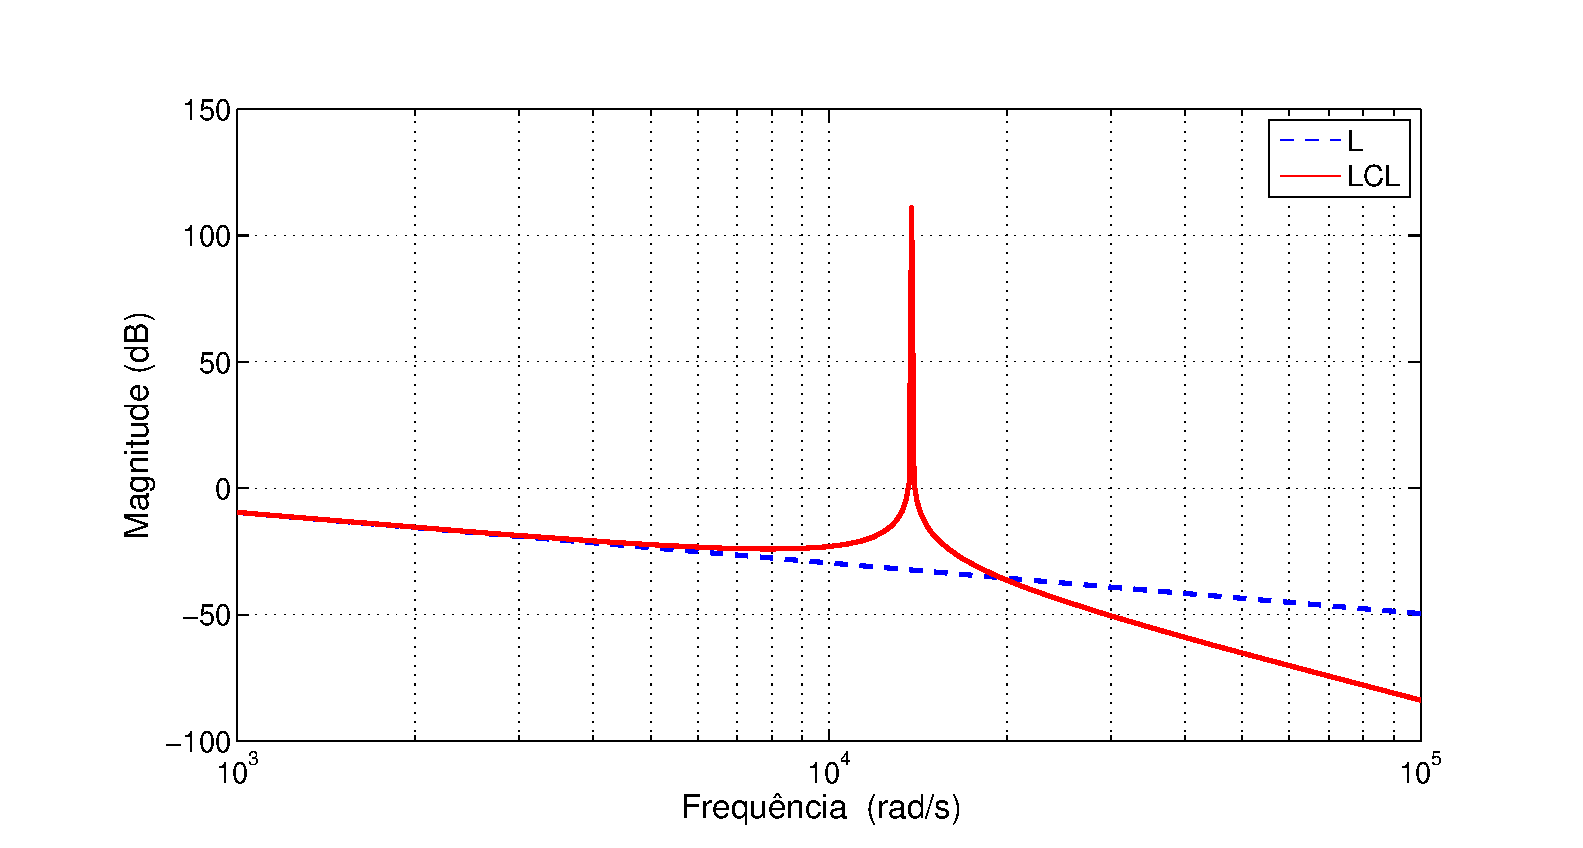
\includegraphics[width=0.9\textwidth]{img/L_vs_LCL}}
    %            \subcaption{Comparação entre filtro L e filtro LCL.}
    %            \label{fig:L_vs_LCL}
    %        \end{minipage}
    %        \begin{minipage}[b]{1\linewidth}
    %            \centering{
    %            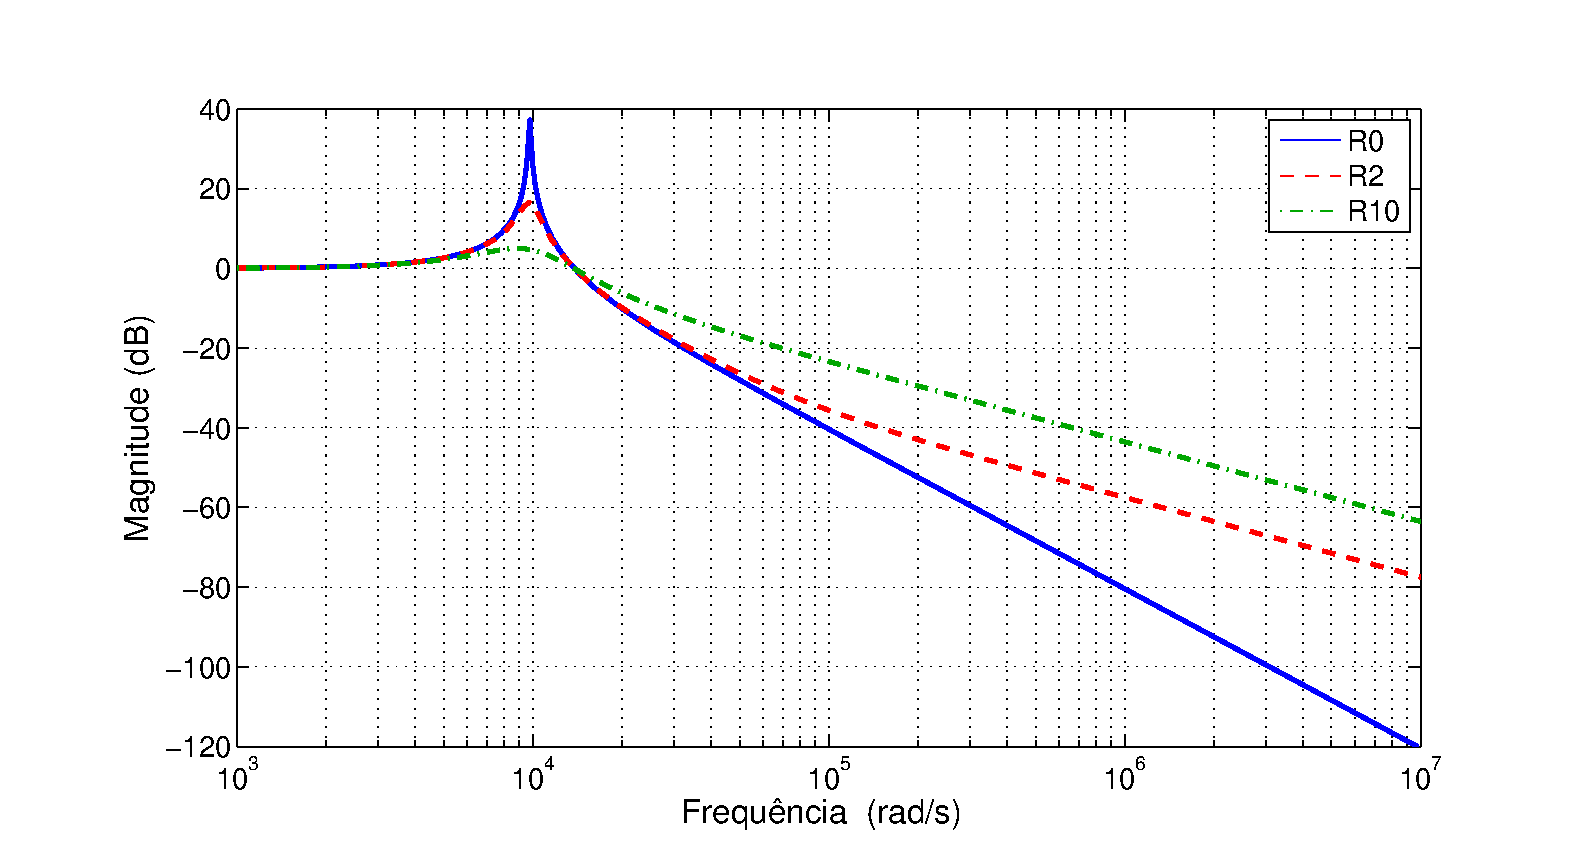
\includegraphics[width=0.9\textwidth]{img/R_in_LCL}}
    %            \subcaption{Efeito do amortecimento passivo.}
    %            \label{fig:R_in_LCL}
    %        \end{minipage}
    %        \renewcommand\figurename{Fig.}
    %        \caption{Diferença entre filtros L, LCL e LCL com amortecimento passivo.}
    %\end{figure}

    \begin{figure}[htb]
        \centering{
            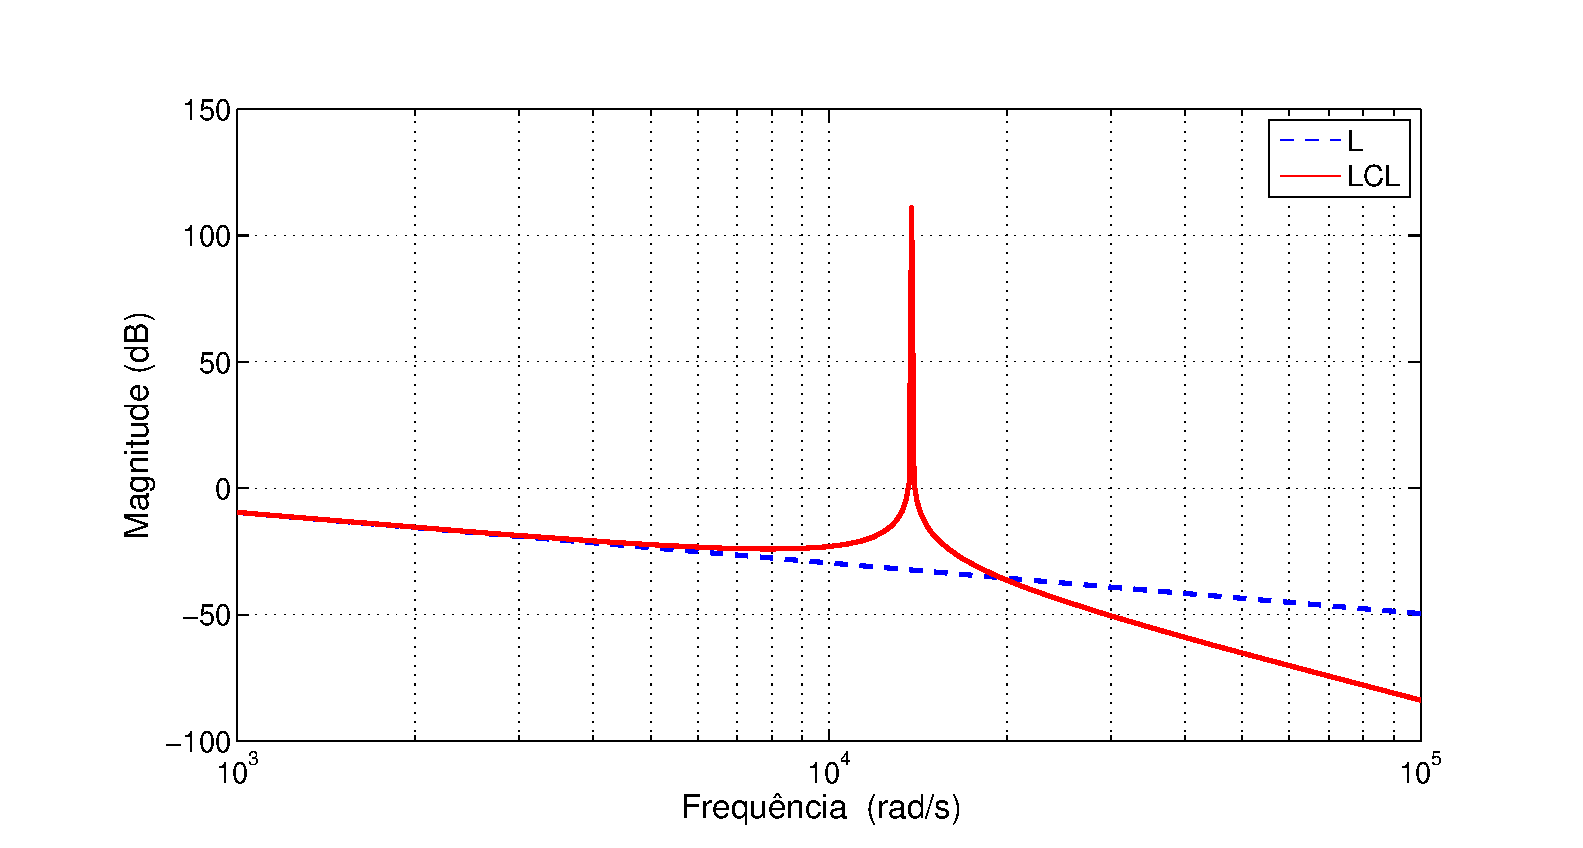
\includegraphics[width=0.9\textwidth]{img/L_vs_LCL}}
        \caption{Comparação entre filtro L e filtro LCL.}
        \label{fig:L_vs_LCL}
    \end{figure}

    A Fig.~\ref{fig:L_vs_LCL} mostra o diagrama de Bode de (\ref{eq:G_v_i2_2})
    com $R_d = 0$ para dois casos: com e sem capacitância $C$. No caso de $C = 0$,
    tem-se o filtro L. No caso de $C \neq 0$, tem-se o filtro LCL.

    Embora nos dois casos a indutância total tenha sido mantida a mesma, observa-se
    que o filtro LCL apresenta uma maior atenuação das harmônicas de comutação
    de alta frequência se comparado ao filtro L. Em contrapartida, o filtro LCL
    possui um pico de amplitude na frequência de ressonância. Por isso, é preciso
    mais cuidado no projeto para manter a estabilidade do sistema.

    O recurso mais comumente utilizado para tal é a adição de um resistor de
    amortecimento $R_d$. O amortecimento passivo, no entanto, reduz a atenuação
    das harmônicas de alta frequência. A Fig.~\ref{fig:R_in_LCL} mostra o diagrama
    de Bode de (\ref{eq:G_i1_i2}) para $R_d = 0$, $R_d = 2$ e $R_d = 10$.

    \begin{figure}[htb]
        \centering{
            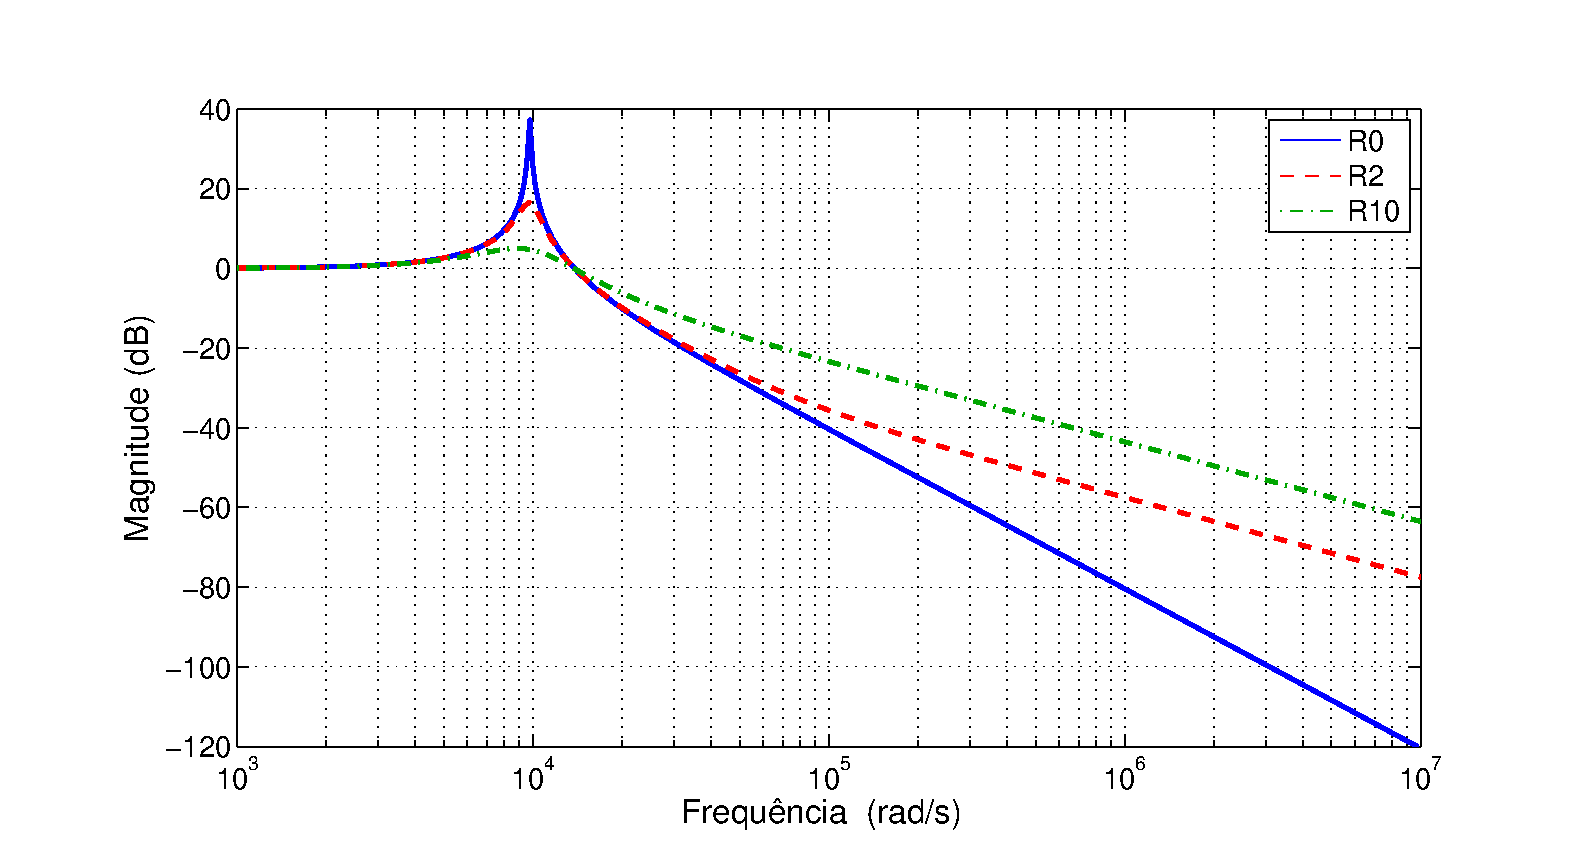
\includegraphics[width=0.9\textwidth]{img/R_in_LCL}}
        \caption{Diferença entre filtros L, LCL e LCL com amortecimento passivo.}
        \label{fig:R_in_LCL}
    \end{figure}

    A redução no amortecimento de harmônicas de alta frequência faz com que filtros
    LCL com amortecimento passivo sejam maiores que filtros LCL sem amortecimento
    passivo, para que atinjam o mesmo desempenho. Esse aumento de tamanho implica
    em aumento de custo e redução da banda passante do filtro.

    As considerações aqui feitas demonstram o porquê da escolha do filtro LCL sem
    amortecimento passivo. Embora seja mais trabalhoso e delicado projetá-lo,
    o desempenho é visivelmente melhor.


\section{Corrente e Tensão do Capacitor}

    O sistema formado pelo conversor alimentado por tensão conectado à rede através
    de um filtro \textit{LCL} é um sistema composto por estados que podem ser
    utilizados em uma estrutura multimalha, onde a malha interna pode ser projetada
    para controlar a tensão ou a corrente do capacitor. Independentemente de qual
    variável é escolhida, o conhecimento da indutância $L_1$ e da capacitância $C$
    do filtro facilitam o projeto da malha interna. Deve haver, no entanto, capacidade
    de rejeição de distúrbios.

    %Comentar que independente de se controlar a tensão ou corrente do capacitor,
    %estas variáveis estão associadas a elementos conhecidos (L1 e C)

    O Controle Multimalha, é adequado para melhorar o desempenho
    de sistemas de controle com apenas uma malha em que o distúrbio esteja
    relacionado com a variável manipulada ou quando o elemento de controle final
    exibe um comportamento não-linear~\cite{ref:LEE}.

    A Fig.~\ref{fig:multiloop} mostra a estrutura geral do Controle Multimalha, onde
    $r_1$ é a referência para a malha externa, $r_2$ é a referência para a malha
    interna, $G_p$ é a função de transferência do controlador primário,
    $G_s$ é a função de transferência do controlador secundário, $P_1$ e $P_2$
    são a planta, $d_1$ e $d_2$ são os distúrbios:

    %\comment{
    %Uma forma
    %de fazer isto é controlar ou a corrente ou a tensão do capacitor. O controle
    %de cada parâmetro tem vantagens sobre o controle do outro, e é necessária
    %uma análise mais aprofundada para verificar qual a melhor opção.
    %}

    \begin{figure}[htb]
        \centering{
            \includegraphics[width=0.9\textwidth]{img/multiloop_geral}}
        \renewcommand\figurename{Fig.}
        \caption{Estrutura geral de Controle Multimalha.}
        \label{fig:multiloop}
    \end{figure}

    A decisão sobre qual variável deve ser controlada em cada uma das malhas é complexa,
    e uma análise mais profunda deve ser feita para verificar qual a melhor
    opção para cada malha. Essa análise é feita em~\cite{ref:NASER}, utilizando o
    método do lugar das raízes e a técnica do espaço de estados médio. Esta é uma técnica
    essencial para a análise de circuitos chaveados, pois permite que as técnicas de
    análise de circuitos tradicionais sejam aplicadas à eles.

    O princípio de funcionamento é que a comutação ciclo à ciclo é ignorada em
    favor das características médias do circuito nas frequências abaixo da
    frequência de Nyquist. Perde-se então a capacidade de ver a forma de onda
    da comutação, mas pode-se determinar rapidamente uma série de fatores
    do circuito, como estabilidade, margem de ganho e de fase, o lugar das
    raízes e a resposta transiente média. Os passos para usar esta técnica são
    os seguintes:

    \begin{enumerate}
        \item Desenhar o circuito em cada estado;
        \item Escrever a equação de nó, malha ou elemento para cada estado;
        \item Determinar qual parcela do período o sistema permanece em cada estado;
        \item Multiplicar cada equação de estado por sua parcela de tempo e somá-las
            para obter uma média ponderada das equações de estado.
    \end{enumerate}

    As funções de transferência da tensão $v_c$ e da corrente $i_c$ do
    capacitor são dadas por:

    \begin{equation}
        v_c = \frac{\frac{2V_{DC}}{L_1} \frac{1}{C} \left( s + \frac{R_2}{L_2} \right)}{s^3 + a_2 s^2 + a_1 s + a_0}
        \label{eq:vc}
    \end{equation}

    \begin{equation}
        i_c = \frac{\frac{2V_{DC}}{L_1} s \left( s + \frac{R_2}{L_2} \right)}{s^3 + a_2 s^2 + a_1 s + a_0}
        \label{eq:ic}
    \end{equation}

    Com

    \begin{equation*}
        a_2 = \frac{R_1}{L_1} + \frac{R_2}{L_2}
    \end{equation*}

    \begin{equation*}
        a_1 = \frac{1}{L_1 L_2} \left( R_1 R_2 + \frac{L_1 + L_2}{C} \right)
    \end{equation*}

    \begin{equation*}
        a_0 = \frac{R_1 + R_2}{C L_1 L_2}
    \end{equation*}

    %\comment{
    %\begin{figure}[htb]
    %        \begin{minipage}[b]{1\linewidth}
    %            \centering{
    %            \includegraphics[width=0.9\textwidth]{img/rlocus_vc}}
    %            \subcaption{Lugar das raízes para a tensão do capacitor.}
    %            \label{fig:rlocus_vc}
    %        \end{minipage}
    %        \begin{minipage}[b]{1\linewidth}
    %            \centering{
    %            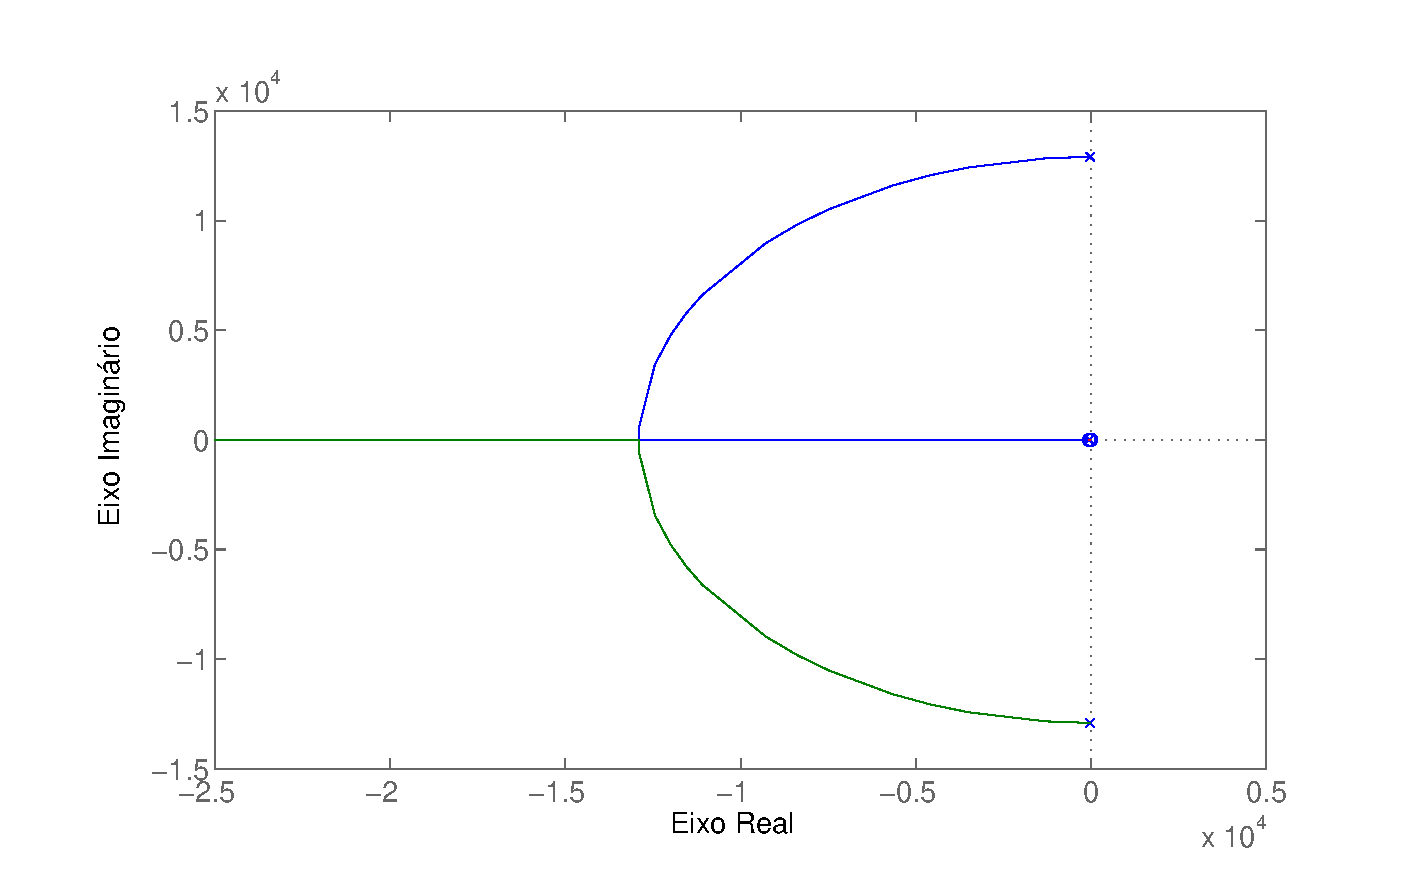
\includegraphics[width=0.9\textwidth]{img/rlocus_ic}}
    %            \subcaption{Lugar das raízes para a corrente do capacitor.}
    %            \label{fig:rlocus_ic}
    %        \end{minipage}
    %        \renewcommand\figurename{Fig.}
    %        \caption{Análise de estabilidade para a corrente e a tensão do capacitor.}
    %\end{figure}
    %}

    A Fig.~\ref{fig:rlocus_vc} mostra o lugar das raízes para a função de
    transferência (\ref{eq:vc}).

    %\comment{
    \begin{figure}[htb]
        \centering{
            \includegraphics[width=0.9\textwidth]{img/rlocus_vc}}
        \renewcommand\figurename{Fig.}
        \caption{Lugar das raízes para a tensão do capacitor.}
        \label{fig:rlocus_vc}
    \end{figure}
    %}

    Percebe-se que os polos da função de transferência da tensão do capacitor
    apresentam um comportamento oscilatório ao longo do eixo imaginário. Devido
    ao projeto do filtro \textit{LCL}, a oscilação não ocorre em uma frequência
    muito alta, o que simplifica o controle desta variável. Além disso, na prática
    haverá sempre parte real nas resistências, o que fará com que os polos desloquem-se
    um pouco para o semiplano esquerdo, saindo do limiar de estabilidade.

    Supondo que o controlador da malha interna tenha um elevado desempenho
    no rastreamento de referências e na rejeição de distúrbios,
    o controle da tensão do capacitor é vantajoso. O capacitor
    pode ser visto como uma fonte de tensão, e toda a dinâmica
    do inversor e do indutor do lado do conversor podem ser ignorados,
    simplificando o controle da corrente da rede.

    A Fig.~\ref{fig:rlocus_ic} mostra o lugar das raízes para a função de
    transferência (\ref{eq:ic}).

    %\comment{
    \begin{figure}[htb]
        \centering{
            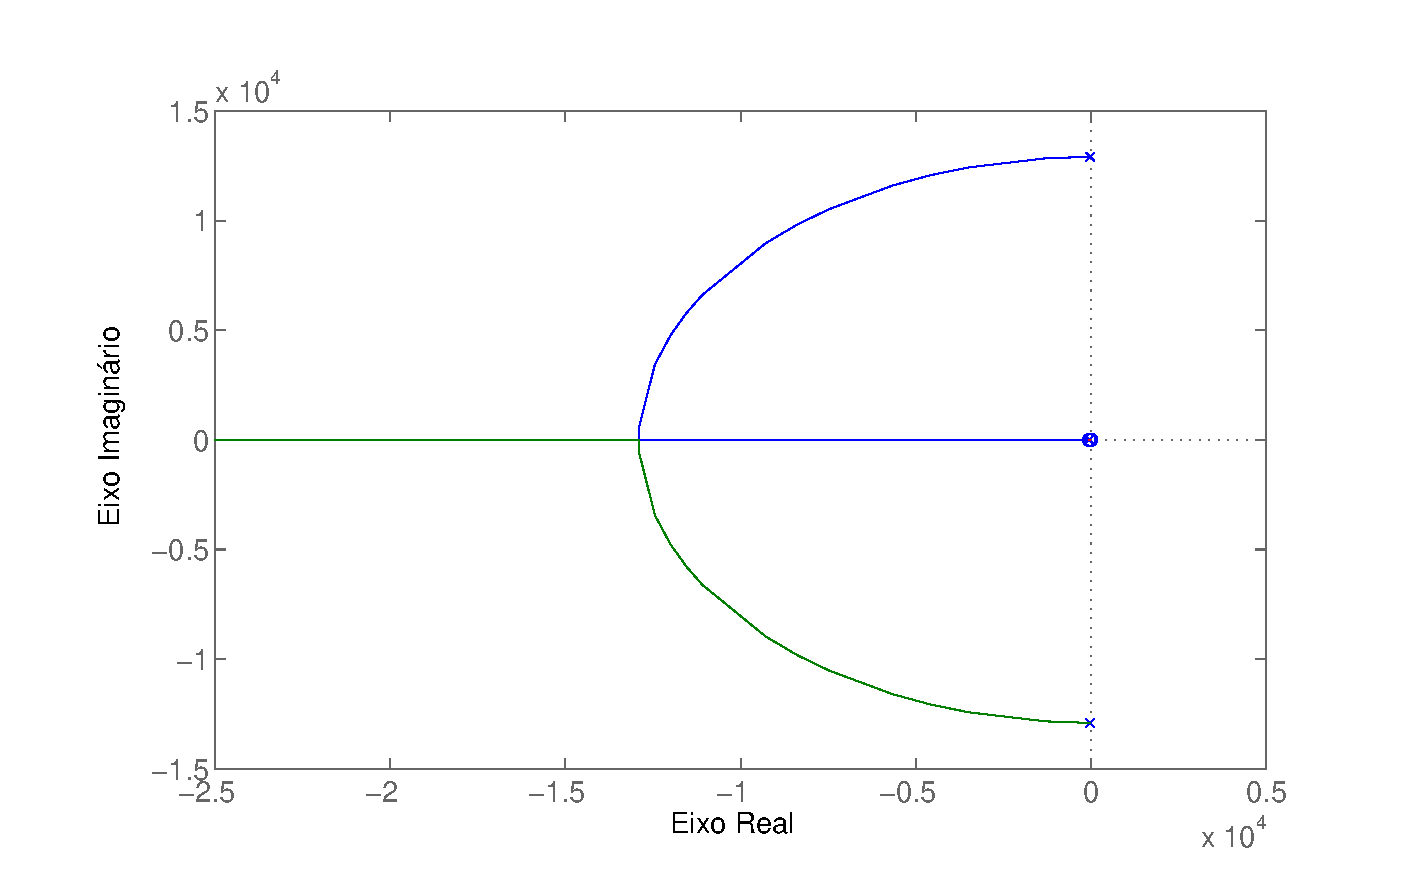
\includegraphics[width=0.9\textwidth]{img/rlocus_ic}}
        \renewcommand\figurename{Fig.}
        \caption{Lugar das raízes para a corrente do capacitor.}
        \label{fig:rlocus_ic}
    \end{figure}
    %}

    Percebe-se que os polos da função de transferência da corrente do capacitor
    deslocam-se para o semiplano esquerdo, indicando que o sistema tende à
    estabilidade. Essa é a grande vantagem de utilizar a corrente do capacitor
    como variável de controle da malha interna.

    A corrente do capacitor mostra-se como uma ótima escolha. No entanto, a tensão
    do capacitor pode ser selecionada como uma variável intermediária a ser controlada,
    sintetizando-se assim uma fonte de tensão controlada por tensão, no caso, o
    conversor. Deste modo, ter-se-á um circuito do tipo \textit{RL} que aproxima o
    comportamento no ponto de conexão.

    Dessa forma, embora a corrente ofereça mais estabilidade, a tensão do capacitor
    é escolhida como variável de controle da malha interna na presença de um controlador
    adaptativo na malha externa, devido ao quanto essa escolha facilita a realização do
    controle da dinâmica do filtro. Outras topologias para a malha externa serão
    avaliadas, e então a corrente do capacitor será utilizada como variável de
    controle para a malha interna.


%FIM---------------------------------------------------------------------------


% ----------------------------------------------------------
% Resultados
% ----------------------------------------------------------
%\part{Resultados}

%TITULO-------------------------------------------------------------------

%=========================================================================
\chapter{Modelagem de Conversores Conectados à Rede Elétrica via Filtro LCL}\label{modelagem}
%=========================================================================

	%intro temporária, melhorar
	Este capítulo apresenta a modelagem de conversores de potência conectados à rede elétrica via filtro LCL. São apresentados modelos dinâmicos e em espaço de estados, bem como em coordenadas $\alpha \beta 0$ \cite{ref:JORGE} e em função de transferência, considerando a corrente $i_C$ e a tensão $v_C$ do capacitor como variável intermediária. Modelos em tempo discreto são desenvolvidos, levando em conta o impacto do atraso de transporte da implementação digital.


\section{Modelo em Espaço de Estados - Coordenadas \emph{abc}}

  Considere um conversor trifásico conectado à rede elétrica via filtro LCL conforme a Fig.~\ref{fig:LCL_topologia_2}. Considere ainda a rede elétrica como sendo uma fonte de tensão trifásica alternada equilibrada com uma impedância série equivalente com característica indutiva.

  \begin{figure}[htb]
    \centering{
      %\includegraphics[width=0.9\textwidth]{img/topologia}}
      \def\svgwidth{\textwidth}
      \input{./img/topologia.pdf_tex}}
    \renewcommand\figurename{Fig.}
    \caption{Topologia do filtro LCL.}
    \label{fig:LCL_topologia_2}
  \end{figure}

  A partir das leis de Kirchhoff pode-se obter:
  %
  \begin{equation}
    u_{ab}(t) = R_1 i_{a1}(t) + L_1 \frac{d}{dt} i_{a1}(t) + v_{an}(t)
      - v_{bn}(t) - L_1 \frac{d}{dt} i_{b1}(t) - R_1 i_{b1}(t) \text{,}
  \end{equation}
  %
  \begin{equation}
    u_{bc}(t) = R_1 i_{b1}(t) + L_1 \frac{d}{dt} i_{b1}(t) + v_{bn}(t)
      - v_{cn}(t) - L_1 \frac{d}{dt} i_{c1}(t) - R_1 i_{c1}(t) \text{,}
  \end{equation}
  %
  \begin{equation}
    i_{a1}(t) + i_{b1}(t) + i_{c1}(t) = 0 \implies \frac{d}{dt} i_{a1}(t)
      + \frac{d}{dt} i_{b1}(t) + \frac{d}{dt} i_{c1}(t) = 0 \text{.}
  \end{equation}

  Além disso, das tensões nos capacitores:
  %
  \begin{equation}
    C \frac{d}{dt} v_{an}(t) = i_{a1}(t) - i_{a2}(t) \text{,}
  \end{equation}
  %
  \begin{equation}
    C \frac{d}{dt} v_{bn}(t) = i_{b1}(t) - i_{b2}(t) \text{,}
  \end{equation}
  %
  \begin{equation}
    C \frac{d}{dt} v_{an}(t) + C \frac{d}{dt} v_{bn}(t) +
      C \frac{d}{dt} v_{cn}(t) = 0 \text{.}
  \end{equation}

  E das correntes do lado da rede:
  %
  \begin{equation}
    v_{ab}(t) = R_2 i_{a2}(t) + L_2 \frac{d}{dt} i_{a2}(t) + v_a(t) - v_b(t)
      - L_2 \frac{d}{dt} i_{b2}(t) - R_2 i_{b2}(t) \text{,}
  \end{equation}
  %
  \begin{equation}
    v_{bc}(t) = R_2 i_{b2}(t) + L_2 \frac{d}{dt} i_{b2}(t) + v_b(t) - v_c(t)
      - L_2 \frac{d}{dt} i_{c2}(t) - R_2 i_{c2}(t) \text{,}
  \end{equation}
  %
  \begin{equation}
    i_{a2}(t) + i_{b2}(t) + i_{c2}(t) = 0 \implies \frac{d}{dt} i_{a2}(t) +
      \frac{d}{dt} i_{b2}(t) + \frac{d}{dt} i_{c2}(t) = 0 \text{.}
  \end{equation}

  É possível escrever esse modelo em forma matricial,
  %
  \begin{equation}
    \begin{split}
      \mathbf{L} \frac{d}{dt} \mathbf{x}_{abc}(t) & = \mathbf{Ax}_{abc}(t) +
          \mathbf{Bu}_{Labc}(t) + \mathbf{Fv}_{abc}(t) \\
      \mathbf{y}(t) & = \mathbf{C}_{abc} \mathbf{x}_{abc}(t) \text{,}
    \end{split}
  \end{equation}
  %
  na qual as variáveis de saída podem ser tanto as correntes do lado do conversor quanto as correntes do lado da rede. A escolha é feita através da matriz $\mathbf{C}_{abc}$. $\mathbf{x}_{abc}(t)$ representa os estados em coordenadas \emph{abc}, $\mathbf{u}_{Labc}(t)$ representa as tensões de linha aplicadas pelo conversor e $\mathbf{v}_{abc}(t)$ representa as tensões de fase da rede.

  Pode-se simplificar o modelo multiplicando por $\mathbf{L}^{-1}$ dos dois lados da igualdade, obtendo
  %
  \begin{equation}
    \begin{split}
      \frac{d}{dt} \mathbf{x}_{abc}(t) & = \mathbf{A}_{abc} \mathbf{x}_{abc}(t) +
        \mathbf{Bu}_{Labc}(t) + \mathbf{F}_{abc} \mathbf{v}_{abc}(t) \\
        \mathbf{y}(t) & = \mathbf{C}_{abc} \mathbf{x}_{abc}(t) \text{.}
    \end{split}
  \end{equation}

  É necessário representar o vetor de tensões do conversor $\mathbf{u}_{Labc}(t)$ em grandezas de fase, o que implica na transformação
  %
  \begin{equation}
    \mathbf{u}_{Labc}(t) = \left[
      \begin{array}{ccc}
        1 &           -1 & \phantom{-}0 \\[0.3em]
        0 & \phantom{-}1 &           -1 \\[0.3em]
        1 & \phantom{-}1 & \phantom{-}1
      \end{array}
    \right] \mathbf{u}_{abc}(t) = \mathbf{T}_{FL} \mathbf{u}_{abc}(t)
  \end{equation}

  Dessa forma, obtem-se
  %
  \begin{equation}
    \begin{split}
      \frac{d}{dt} \mathbf{x}_{abc}(t) & = \mathbf{A}_{abc} \mathbf{x}_{abc}(t) +
        \mathbf{BT}_{FL} \mathbf{u}_{abc}(t) + \mathbf{F}_{abc} \mathbf{v}_{abc}(t) \\
      \mathbf{y}(t) & = \mathbf{C}_{abc} \mathbf{x}_{abc}(t) \text{,}
    \end{split}
  \end{equation}
  %
  que é equivalente a
  %
  \begin{equation}
    \begin{split}
      \frac{d}{dt} \mathbf{x}_{abc}(t) & = \mathbf{A}_{abc} \mathbf{x}_{abc}(t) +
        \mathbf{B}_{abc} \mathbf{u}_{abc}(t) + \mathbf{F}_{abc} \mathbf{v}_{abc}(t) \\
        \mathbf{y}(t) & = \mathbf{C}_{abc} \mathbf{x}_{abc}(t) \text{.}
    \end{split}
    \label{eq:LCL_abc_espaco_estados}
  \end{equation}

  O modelo (\ref{eq:LCL_abc_espaco_estados}) apresenta acoplamento entre as variáveis de cada fase, o que dificulda a sua utilização em sistemas de controle. Devido à isso, uma transformação para desacoplamento é apresentada na seção seguinte.

\section{Modelo em Espaço de Estados - Coordenadas $\alpha \beta 0$}

  A representação de sistemas elétricos trifásicos é objeto de estudos desde o início de sua utilização, no começo do século XX. Dentre as primeiras contribuições neste sentido, encontra-se o trabalho de Charles L. Fortescue~\cite{ref:FORTESCUE}, conhecido como a teoria de componentes simétricas, que representa um sistema trifásico desequilibrado em termos de três sistemas trifásicos equilibrados, chamados circuitos de sequência positiva, negativa e zero. Uma outra contribuição foi feita por Edith Clarke, com a transformação nomeada em sua homenagem~\cite{ref:CLARKE}. A transformação de Clarke, ou transformação $\alpha \beta 0$ permite representar um sistema trifásico acoplado em termos de componentes monofásicas desacopladas. Essa transformação é muito útil em aplicações de conversores estáticos trifásicos, visto que possibilita a simplificação dos modelos e do projeto dos controladores.

  A transformação $\alpha \beta 0$ é linear e invariante no tempo, e é dada por
  %
  %usando array e phantom{-} pelo alinhamento
  \begin{equation}
    \mathbf{T}_{\alpha \beta 0} = \frac{2}{3} \left[
    \begin{array}{ccc}
      1 & -\frac{1}{2} & -\frac{1}{2} \\[0.3em]
      0 & \phantom{-}\frac{\sqrt{3}}{2} & -\frac{\sqrt{3}}{2} \\[0.3em]
      \frac{1}{2} &  \phantom{-}\frac{1}{2} & \phantom{-}\frac{1}{2}
    \end{array}
    \right] \text{.}
    \label{eq:alpha_beta_0}
  \end{equation}

  Utilizando essa transformação, qualquer parâmetro em coordenadas $abc$ pode ser transcrito em coordenadas $\alpha \beta 0$, e vice versa
  %
  \begin{equation}
    \mathbf{T}_{\alpha \beta 0} \mathbf{x}_{abc} = \mathbf{x}_{\alpha \beta 0}
    \iff
    \mathbf{T}_{\alpha \beta 0}^{-1} \mathbf{x}_{\alpha \beta 0} = \mathbf{x}_{abc}
    \text{.}
  \end{equation}

  No projeto de controladores para sistemas elétricos trifásicos, é usual levar em consideração essa transformação e modelar o sistema para o caso monofásico, projetando o controlador considerando os equivalentes nas coordenadas $\alpha$ e $\beta$. A Fig~\ref{fig:LCL_geral} apresenta a estrutura do sistema para o caso monofásico. Neste caso, as indutâncias do filtro são: $L_1$ do lado do conversor e $L_2$ do lado da rede, $C$ é a capacitância do filtro e $L_g$ é a indutância da rede elétrica. A tensão gerada pelo conversor é representada por $u_{\alpha}$ e a rede elétrica é representada por
  $v_{\alpha}$.

  \begin{figure}[htb]
    \centering{
      %\includegraphics[width=0.9\textwidth]{img/LCL_geral}}
      \def\svgwidth{\textwidth}
      \input{./img/LCL_geral.pdf_tex}}
    \renewcommand\figurename{Fig.}
    \caption{Filtro LCL para o caso monofásico.}
    \label{fig:LCL_geral}
  \end{figure}

  Visto que a transformação (\ref{eq:alpha_beta_0}) é invariante no tempo, ela pode ser aplicada ao modelo (\ref{eq:LCL_abc_espaco_estados}). Dessa forma, tem-se que
  %
  \begin{equation}
    \begin{split}
      \mathbf{T}_{\alpha \beta 0} \frac{d}{dt} \mathbf{x}_{abc}(t) & =
        \mathbf{T}_{\alpha \beta 0} \mathbf{A}_{abc} \mathbf{x}_{abc}(t) +
        \mathbf{T}_{\alpha \beta 0} \mathbf{B}_{abc} \mathbf{u}_{abc}(t) +
        \mathbf{T}_{\alpha \beta 0} \mathbf{F}_{abc} \mathbf{v}_{abc}(t) \\
      \mathbf{T}_{\alpha \beta 0} \mathbf{y}_{abc}(t) & =
        \mathbf{T}_{\alpha \beta 0} \mathbf{C}_{abc} \mathbf{x}_{abc}(t) \text{,}
    \end{split}
  \end{equation}
  %
  isto é,
  %
  \begin{equation}
    \begin{split}
      \frac{d}{dt} \mathbf{x}_{\alpha \beta 0}(t) & =
        \mathbf{A}_{\alpha \beta 0} \mathbf{x}_{\alpha \beta 0}(t) +
        \mathbf{B}_{\alpha \beta 0} \mathbf{u}_{\alpha \beta 0}(t) +
        \mathbf{F}_{\alpha \beta 0} \mathbf{v}_{\alpha \beta 0}(t) \\
      \mathbf{y}_{\alpha \beta 0}(t) & = \mathbf{C}_{\alpha \beta 0}
        \mathbf{x}_{\alpha \beta 0}(t) \text{.}
    \end{split}
    \label{eq:LCL_ab0_espaco_estados}
  \end{equation}

  O modelo (\ref{eq:LCL_ab0_espaco_estados}) representa o sistema na forma de dois sistemas monofásicos desacoplados associados ao eixo $\alpha$ e ao eixo $\beta$. O eixo $0$ pode ser desconsiderado, já que não há caminho para circulação de corrente de sequência zero.

\section{Modelo em Função de Transferência}

  Uma forma conveniente de modelar o sistema é através de impedâncias complexas~\cite{ref:XU}. As indutâncias e a capacitância do filtro podem ser representadas pelas seguintes impedâncias
  %
  \begin{equation}
    \begin{split}
      Z_i & = r_1 + L_1 s \text{,} \\
      Z_C & = \frac{1}{s C} \text{,} \\
      Z_g & = r_2 + r_g + \left( L_2 + L_g \right) s \text{.}
    \end{split}
  \end{equation}

  A impedância do lado da rede $Z_g$ engloba duas indutâncias: uma indutância projetada, $L_2$, e uma indutância desconhecida que é a indutância da rede elétrica $L_g$. Escolheu-se essa forma de representação de modo a explicitar a incerteza paramétrica, apesar de $L_2$ ser uma indutância projetada. Além disso, é importante esclarecer que a tensão da rede $v_g$ pode ser desprezada na obtenção do modelo, visto que é um distúrbio exógeno que deve ser rejeitado pelo controlador adaptativo.

  % A Fig.~\ref{fig:estrutura_geral_cascata} demonstra a estrutura de controle utilizada.

  % \begin{figure}[htb]
  %     \centering{
  %         %\includegraphics[width=0.9\textwidth]{img/cascade_general}}
  %         \def\svgwidth{0.9\textwidth}
  %         \input{./img/multiloop_geral.pdf_tex}}
  %     \renewcommand\figurename{Fig.}
  %     \caption{Diagrama de blocos demonstrando a estrutura geral de controle.}
  %     \label{fig:estrutura_geral_cascata}
  % \end{figure}

  % Observa-se que $U_p$ indica a variável de controle intermediária utilizada para implementar a malha interna e realizar o amortecimento ativo da ressonância do filtro, podendo ser $V_C$ ou $I_C$. O controlador adaptativo na malha externa gera a referência $U$ para a malha interna, que por sua vez gera a ação de controle $U_c$ implementada via PWM.

  Considerando a estrutura da Fig.~\ref{fig:LCL_geral} e desprezando o distúrbio da rede $v_g$, obtém-se as seguintes expressões a partir das leis de Kirchhoff
  %
  \begin{equation}
    \frac{V_C}{U_c} = \frac{Z_C Z_g}{Z_i \left( Z_C + Z_g \right) + Z_C Z_g}
    \text{,}
    \label{eq:vc_uc}
  \end{equation}
  %
  \begin{equation}
    \frac{I_C}{U_c} = \frac{Z_g}{Z_i \left( Z_C + Z_g \right) + Z_C Z_g}
    \text{,}
    \label{eq:ic_uc}
  \end{equation}
  %
  \begin{equation}
    \frac{I_2}{U_c} = \frac{Z_C}{Z_i \left( Z_C + Z_g \right) + Z_C Z_g}
    \text{.}
  \end{equation}

  Do ponto de vista de amortecimento ativo, todo e qualquer elemento resistivo que se encontre no sistema irá colaborar com o amortecimento, embora de forma passiva. Por esse motivo, as resistências são desprezadas na modelagem do sistema, visto que isto irá facilitar a modelagem e criar um caso pior do que o que se encontra na prática.

  A discretização destas funções de transferência é feita conforme realizado em \cite{ref:PARKER}, incluindo um retentor de ordem zero (ZOH) e aplicando a transformada $\mathcal{Z}$. Dessa forma, considerando o atraso de tempo associado à implementação digital, obtém-se
  %
  \begin{equation}
    G_d (z) = \frac{I_2}{U_c} = K_1 \frac{1}{z \left( z-1 \right)}
    - \frac{K_1 \sen \left( \omega_n T_s \right) }{\omega_n T_s}
    \frac{z-1}{z \left( z^2 - 2 \cos\left( \omega_n T_s \right) z +1 \right) }
    \text{,}
  \end{equation}
  %
  onde $T_s$ é o período de amostragem e
  %
  \begin{equation}
    K_1 = \frac{T_s}{L1 + L2 + Lg} \text{,}
  \end{equation}
  %
  \begin{equation}
    \omega_n = \sqrt{\frac{ L_1 + L_2 + L_g }{ L_1 C \left( L_2 + L_g \right)}}
    \text{.}
  \end{equation}

  No caso em que a variável intermediária é a tensão do capacitor $V_C$, para relacionar $I_2$ com $V_C$ é necessário discretizar a equação~(\ref{eq:vc_uc})
  %
  \begin{equation}
    G_{id_{vc}}(z) = \frac{2 \sen^2 \left( \omega_n \frac{T_s}{2} \right)}{L_1 C \omega_n^2}
      \frac{z+1}{z \left( z^2 - \cos \left( \omega_n T_s \right) z + 1 \right)}
      \text{.}
  \end{equation}

  Dessa forma, a relação $G_{od_{vc}}$ entre $I_2$ e $V_C$ é
  %
  \begin{equation}
    G_{od_{vc}}(z) = \frac{I_2}{V_C} = \frac{G_d}{G_{id_{vc}}} \text{.}
    \label{eq:god_i2_vc}
  \end{equation}

  De forma semelhante, no caso em que a variável intermediária é a corrente do capacitor $I_C$, para relacionar $I_2$ com $I_C$ é necessário discretizar a equação~(\ref{eq:ic_uc})
  %
  \begin{equation}
    G_{id_{ic}}(z) = \frac{\sen \left( \omega_n T_s \right)}{\omega_n L_1}
      \frac{z-1}{z \left( z^2 - \cos \left( \omega_n T_s \right) z + 1 \right)}
      \text{,}
  \end{equation}
  %
  e assim
  %
  \begin{equation}
    G_{od_{ic}}(z) = \frac{I_2}{I_C} = \frac{G_d}{G_{id_{ic}}} \text{.}
    \label{eq:god_i2_ic}
  \end{equation}


\section{Efeitos da Discretização}

  Plantas de fase mínima, ou seja, aquelas que apresentam zeros apenas no semi-plano esquerdo do plano $s$, permitem que os efeitos de zeros indesejados sejam cancelados pela alocação de pólos do controlador. Isso é impossível, no entanto, no caso de plantas de fase não-mínima, visto que a alocação de pólos do controlador no semi-plano esquerdo resulta em instabilidade.

  Por isso, é importante observar que a discretização de um sistema pode implicar em problemas do ponto de vista de controle. Mesmo uma planta de fase mínima em tempo contínuo pode apresentar zeros de fase não-mínima após a discretização. De fato, de uma forma mais geral, plantas em tempo contínuo com grau relativo $n \ge 2$ apresentam zeros de discretização \cite{ref:ASTROM}. Esse é o caso do filtro LCL quando a variável controlada é a corrente do lado da rede.

  %Para fazer subreferências:
  %
  %As figuras \ref{fig:pzmap_ic_vc_d}.\subref{fig:pzmap_ic} e \ref{fig:pzmap_ic_vc_d}.\subref{fig:pzmap_vc} apresentam o diagrama de pólos e zeros para o filtro LCL e demonstram esse efeito.

  A Fig.~\ref{fig:pzmap_ic_vc} apresenta o diagrama de pólos e zeros para a planta contínua. A Fig.~\ref{fig:pzmap_ic_vc_d} apresenta o diagrama de pólos e zeros para a planta discreta, evidenciando o surgimento de um zero fora do círculo de raio unitário. Este é um zero instável inerentemente introduzido pelo processo de discretização.

  \begin{figure}[htb]
    \centering
    \raisebox{-0.5\height}{
      \def\svgwidth{0.8\textwidth}
      \input{./img/logo.pdf_tex}}
    \caption{Diagrama de pólos e zeros para o filtro LCL em tempo contínuo.}
    \label{fig:pzmap_ic_vc}
  \end{figure}

  \begin{figure}[htb]
    \centering
    \subfloat[Corrente do capacitor.]{\label{fig:pzmap_ic_d}
      {\input{./img/pzmap_ic.tex}}}\\
    \subfloat[Tensão do capacitor.]{\label{fig:pzmap_vc_d}
      {% This file was created by matlab2tikz v0.4.7 running on MATLAB 7.14.
% Copyright (c) 2008--2014, Nico Schlömer <nico.schloemer@gmail.com>
% All rights reserved.
% Minimal pgfplots version: 1.3
% 
% The latest updates can be retrieved from
%   http://www.mathworks.com/matlabcentral/fileexchange/22022-matlab2tikz
% where you can also make suggestions and rate matlab2tikz.
% 
%
% defining custom colors
\definecolor{mycolor1}{rgb}{0.66667,0.66667,0.66667}%
%
\begin{tikzpicture}

\begin{axis}[%
width=0.8\textwidth,
height=0.461611624834875\textwidth,
scale only axis,
xmin=-4,
xmax=1.2,
xtick={-4, -3, -2, -1,  0,  1},
xlabel={Eixo Real},
ymin=-1.4,
ymax=1.4,
ytick={-1,  0,  1},
ylabel={Eixo Imaginário}
]
\addplot [color=mycolor1,dotted,line width=1.0pt,forget plot]
  table[row sep=crcr]{1	0\\
0.987688340595138	0.156434465040231\\
0.951056516295154	0.309016994374947\\
0.891006524188368	0.453990499739547\\
0.809016994374947	0.587785252292473\\
0.707106781186548	0.707106781186547\\
0.587785252292473	0.809016994374947\\
0.453990499739547	0.891006524188368\\
0.309016994374947	0.951056516295154\\
0.156434465040231	0.987688340595138\\
6.12323399573677e-17	1\\
-0.156434465040231	0.987688340595138\\
-0.309016994374947	0.951056516295154\\
-0.453990499739547	0.891006524188368\\
-0.587785252292473	0.809016994374947\\
-0.707106781186547	0.707106781186548\\
-0.809016994374947	0.587785252292473\\
-0.891006524188368	0.453990499739547\\
-0.951056516295154	0.309016994374948\\
-0.987688340595138	0.156434465040231\\
-1	1.22464679914735e-16\\
};
\addplot [color=mycolor1,dotted,line width=1.0pt,forget plot]
  table[row sep=crcr]{1	0\\
0.972218045703082	0.153984211042097\\
0.921496791140463	0.299412457456957\\
0.849791018366557	0.432990150609548\\
0.759508516401756	0.551815237548133\\
0.653437051516106	0.653437051516106\\
0.534664304371591	0.735902282058355\\
0.406492952796512	0.797787339572243\\
0.272353130096494	0.83821674479613\\
0.135714483753824	0.856867527364047\\
5.22899666167123e-17	0.853959960588124\\
-0.131496350792703	0.830235283991667\\
-0.255686250369537	0.786921363444393\\
-0.369756251949576	0.725687504552447\\
-0.47122811850853	0.648589862732789\\
-0.558009078759514	0.558009078759514\\
-0.628431083783263	0.456581908289041\\
-0.681278445058817	0.347128705949459\\
-0.715803538350409	0.232578668243255\\
-0.731730559897045	0.115894735197653\\
-0.729247614287671	8.9307075662324e-17\\
};
\addplot [color=mycolor1,dotted,line width=1.0pt,forget plot]
  table[row sep=crcr]{1	0\\
0.956521682769877	0.151498151383791\\
0.891982039736211	0.289822533396298\\
0.809292583610082	0.412355167436434\\
0.711634858347723	0.517032989000692\\
0.602364630186427	0.602364630186426\\
0.484917701774751	0.667431957639199\\
0.362719588349683	0.711877274647591\\
0.239101059900595	0.735877395777214\\
0.117221283062812	0.740106053489981\\
4.44354699422903e-17	0.725686295399261\\
-0.109940132237539	0.694134676438339\\
-0.210320240583588	0.647299141978847\\
-0.299240493845688	0.587292536894097\\
-0.375203754387119	0.516423664031337\\
-0.437127756959533	0.437127756959533\\
-0.484346224770267	0.351898130574443\\
-0.516599582217932	0.263220634338226\\
-0.534016141209622	0.173512362385299\\
-0.537084820159711	0.0850658786478001\\
-0.526620599330303	6.44924231334916e-17\\
};
\addplot [color=mycolor1,dotted,line width=1.0pt,forget plot]
  table[row sep=crcr]{1	0\\
0.940082788364644	0.148894486293864\\
0.86158608093073	0.279946287694513\\
0.768279786681378	0.391458103646313\\
0.663960650859636	0.482395649771645\\
0.552351927561387	0.552351927561387\\
0.437014383712816	0.601498696728173\\
0.321269860940431	0.630527604183869\\
0.208138182971344	0.640583459188477\\
0.100287778328637	0.633192112325829\\
3.73630739569174e-17	0.610185303761559\\
-0.0908532273476425	0.573624701779294\\
-0.170819110593797	0.525727164509449\\
-0.238861981883349	0.468793035010043\\
-0.294350736089166	0.40513903143051\\
-0.337037028702328	0.337037028702328\\
-0.367025664975262	0.266659754473976\\
-0.384738677688982	0.196034147687371\\
-0.390874612629551	0.127002860400749\\
-0.386364521398959	0.0611941284830315\\
-0.372326104926586	4.55967972637346e-17\\
};
\addplot [color=mycolor1,dotted,line width=1.0pt,forget plot]
  table[row sep=crcr]{1	0\\
0.922246029428501	0.146069421212559\\
0.829201462983264	0.269423887468404\\
0.725373165529273	0.369596088217499\\
0.614985835074999	0.446813363302878\\
0.501902475185001	0.501902475185001\\
0.38956496084428	0.536190168955128\\
0.280953750703967	0.551402782692681\\
0.178565395716864	0.549567778706978\\
0.0844061798404073	0.532919645815306\\
3.08495992433718e-17	0.50381218919366\\
-0.0735915548753502	0.464638791061534\\
-0.135739038566523	0.417761804348184\\
-0.186207014322272	0.365451842507638\\
-0.225110018726605	0.309837359892227\\
-0.252864584784672	0.252864584784672\\
-0.270139142845401	0.196267575756099\\
-0.277803443075876	0.141547924204336\\
-0.27687894570066	0.0899634229303457\\
-0.268491413422519	0.0425248622468694\\
-0.253826721980109	3.10848082611005e-17\\
};
\addplot [color=mycolor1,dotted,line width=1.0pt,forget plot]
  table[row sep=crcr]{1	0\\
0.902056570675584	0.142871725087523\\
0.793293726869509	0.257756756757911\\
0.678769666307395	0.345850419328459\\
0.562876391436159	0.408953636388562\\
0.449318435861499	0.449318435861499\\
0.341115747349381	0.469505547439701\\
0.24062663375655	0.472256359314945\\
0.149586755320764	0.460380694230177\\
0.069160331541479	0.436661148025441\\
2.47240337905553e-17	0.403774113610049\\
-0.057687904157153	0.364227092250654\\
-0.104075505986926	0.320311471399148\\
-0.139645446506012	0.274069620358657\\
-0.165124892040398	0.227274916024158\\
-0.18142315316863	0.18142315316863\\
-0.189574186252466	0.137733708524426\\
-0.190684892879101	0.0971588057560207\\
-0.185889806735969	0.0603992595374446\\
-0.176312467991919	0.0279251515651378\\
-0.16303353482158	1.99658496572927e-17\\
};
\addplot [color=mycolor1,dotted,line width=1.0pt,forget plot]
  table[row sep=crcr]{1	0\\
0.877921760602431	0.139049146701748\\
0.751411952540787	0.244148543365328\\
0.625732257688895	0.318826509862098\\
0.505011411193747	0.36691226736026\\
0.392341669548685	0.392341669548685\\
0.289890514921595	0.399000063654162\\
0.199020572856858	0.390599867100522\\
0.120411913496453	0.370589763847805\\
0.0541820486548744	0.34209199176291\\
1.88512313530119e-17	0.307863971328499\\
-0.042808222513439	0.270280479734772\\
-0.075164540154518	0.231332667812908\\
-0.0981551954909503	0.192640417840451\\
-0.112959067758674	0.155474818616317\\
-0.120787864504912	0.120787864504912\\
-0.122837744156894	0.0892468451742257\\
-0.120251626285951	0.0612712639357851\\
-0.114091236431876	0.0370704898842818\\
-0.105317799143806	0.0166807006736036\\
-0.0947802248421549	1.16072298975411e-17\\
};
\addplot [color=mycolor1,dotted,line width=1.0pt,forget plot]
  table[row sep=crcr]{1	0\\
0.84674396664984	0.134111069256013\\
0.698989566160914	0.227115477506975\\
0.561406498364893	0.286050898428465\\
0.437004973478602	0.317502698182059\\
0.327450698344114	0.327450698344114\\
0.233352139914598	0.321181666481713\\
0.154515499860225	0.303253743289057\\
0.0901653834921457	0.27750051639687\\
0.0391311034995635	0.247064063991275\\
1.31311479217367e-17	0.214447919692096\\
-0.0287598398096346	0.181582482159892\\
-0.0487044416812479	0.149896858349689\\
-0.0613430200940395	0.120392455675976\\
-0.06808779312177	0.0937148074575858\\
-0.0702211210616195	0.0702211210616195\\
-0.068876740220244	0.0500418809603846\\
-0.0650321343871793	0.0331355275052096\\
-0.0595094084547913	0.0193357789181307\\
-0.0529823745536039	0.00839158374073751\\
-0.0459879102602678	5.63189470997126e-18\\
};
\addplot [color=mycolor1,dotted,line width=1.0pt,forget plot]
  table[row sep=crcr]{1	0\\
0.801053465278425	0.126874404768154\\
0.625589539649299	0.203266363189334\\
0.475341369738971	0.242198525079547\\
0.350045057714404	0.254322621147605\\
0.24813777530853	0.24813777530853\\
0.167289292234614	0.230253957320141\\
0.104794333468008	0.205670459781722\\
0.0578515468028918	0.178048753195384\\
0.0237523524567972	0.149966451301199\\
7.54043881219821e-18	0.123144711070133\\
-0.0156239119173694	0.0986454975334405\\
-0.0250311775652273	0.0770380431086105\\
-0.0298254673925332	0.0585357756361869\\
-0.0313184856998208	0.0431061974937683\\
-0.0305568546459545	0.0305568546459545\\
-0.0283545570469435	0.0206007915573586\\
-0.0253272293454815	0.012904867916705\\
-0.021925762268643	0.00712411201600239\\
-0.0184675753156993	0.00292497658052826\\
-0.0151646198645466	1.85713031774033e-18\\
};
\addplot [color=mycolor1,dotted,line width=1.0pt,forget plot]
  table[row sep=crcr]{1	0\\
0.714110955679367	0.113104064044896\\
0.497161927717827	0.161537702532642\\
0.336758208677056	0.171586877647116\\
0.221075553032581	0.160620791180475\\
0.139705610200823	0.139705610200823\\
0.0839640345306934	0.115566579097864\\
0.0468885871776745	0.0920240337831981\\
0.0230753615892199	0.0710186604775083\\
0.00844586939409394	0.0533251206797082\\
2.39022368106624e-18	0.0390353150431684\\
-0.00441505277265522	0.0278755461307222\\
-0.00630567510971132	0.0194068724759343\\
-0.00669794782622876	0.0131454627690819\\
-0.0062698831862128	0.00862975386096949\\
-0.0054534525074872	0.0054534525074872\\
-0.00451117782354635	0.00327756254020109\\
-0.00359218715027031	0.00183031077240959\\
-0.00277223578568335	0.000900754009370227\\
-0.00208156288544739	0.000329687172611911\\
-0.00152375582051941	1.86606268828125e-19\\
};
\addplot [color=mycolor1,dotted,line width=1.0pt,forget plot]
  table[row sep=crcr]{1	-0\\
0.987688340595138	-0.156434465040231\\
0.951056516295154	-0.309016994374947\\
0.891006524188368	-0.453990499739547\\
0.809016994374947	-0.587785252292473\\
0.707106781186548	-0.707106781186547\\
0.587785252292473	-0.809016994374947\\
0.453990499739547	-0.891006524188368\\
0.309016994374947	-0.951056516295154\\
0.156434465040231	-0.987688340595138\\
6.12323399573677e-17	-1\\
-0.156434465040231	-0.987688340595138\\
-0.309016994374947	-0.951056516295154\\
-0.453990499739547	-0.891006524188368\\
-0.587785252292473	-0.809016994374947\\
-0.707106781186547	-0.707106781186548\\
-0.809016994374947	-0.587785252292473\\
-0.891006524188368	-0.453990499739547\\
-0.951056516295154	-0.309016994374948\\
-0.987688340595138	-0.156434465040231\\
-1	-1.22464679914735e-16\\
};
\addplot [color=mycolor1,dotted,line width=1.0pt,forget plot]
  table[row sep=crcr]{1	-0\\
0.972218045703082	-0.153984211042097\\
0.921496791140463	-0.299412457456957\\
0.849791018366557	-0.432990150609548\\
0.759508516401756	-0.551815237548133\\
0.653437051516106	-0.653437051516106\\
0.534664304371591	-0.735902282058355\\
0.406492952796512	-0.797787339572243\\
0.272353130096494	-0.83821674479613\\
0.135714483753824	-0.856867527364047\\
5.22899666167123e-17	-0.853959960588124\\
-0.131496350792703	-0.830235283991667\\
-0.255686250369537	-0.786921363444393\\
-0.369756251949576	-0.725687504552447\\
-0.47122811850853	-0.648589862732789\\
-0.558009078759514	-0.558009078759514\\
-0.628431083783263	-0.456581908289041\\
-0.681278445058817	-0.347128705949459\\
-0.715803538350409	-0.232578668243255\\
-0.731730559897045	-0.115894735197653\\
-0.729247614287671	-8.9307075662324e-17\\
};
\addplot [color=mycolor1,dotted,line width=1.0pt,forget plot]
  table[row sep=crcr]{1	-0\\
0.956521682769877	-0.151498151383791\\
0.891982039736211	-0.289822533396298\\
0.809292583610082	-0.412355167436434\\
0.711634858347723	-0.517032989000692\\
0.602364630186427	-0.602364630186426\\
0.484917701774751	-0.667431957639199\\
0.362719588349683	-0.711877274647591\\
0.239101059900595	-0.735877395777214\\
0.117221283062812	-0.740106053489981\\
4.44354699422903e-17	-0.725686295399261\\
-0.109940132237539	-0.694134676438339\\
-0.210320240583588	-0.647299141978847\\
-0.299240493845688	-0.587292536894097\\
-0.375203754387119	-0.516423664031337\\
-0.437127756959533	-0.437127756959533\\
-0.484346224770267	-0.351898130574443\\
-0.516599582217932	-0.263220634338226\\
-0.534016141209622	-0.173512362385299\\
-0.537084820159711	-0.0850658786478001\\
-0.526620599330303	-6.44924231334916e-17\\
};
\addplot [color=mycolor1,dotted,line width=1.0pt,forget plot]
  table[row sep=crcr]{1	-0\\
0.940082788364644	-0.148894486293864\\
0.86158608093073	-0.279946287694513\\
0.768279786681378	-0.391458103646313\\
0.663960650859636	-0.482395649771645\\
0.552351927561387	-0.552351927561387\\
0.437014383712816	-0.601498696728173\\
0.321269860940431	-0.630527604183869\\
0.208138182971344	-0.640583459188477\\
0.100287778328637	-0.633192112325829\\
3.73630739569174e-17	-0.610185303761559\\
-0.0908532273476425	-0.573624701779294\\
-0.170819110593797	-0.525727164509449\\
-0.238861981883349	-0.468793035010043\\
-0.294350736089166	-0.40513903143051\\
-0.337037028702328	-0.337037028702328\\
-0.367025664975262	-0.266659754473976\\
-0.384738677688982	-0.196034147687371\\
-0.390874612629551	-0.127002860400749\\
-0.386364521398959	-0.0611941284830315\\
-0.372326104926586	-4.55967972637346e-17\\
};
\addplot [color=mycolor1,dotted,line width=1.0pt,forget plot]
  table[row sep=crcr]{1	-0\\
0.922246029428501	-0.146069421212559\\
0.829201462983264	-0.269423887468404\\
0.725373165529273	-0.369596088217499\\
0.614985835074999	-0.446813363302878\\
0.501902475185001	-0.501902475185001\\
0.38956496084428	-0.536190168955128\\
0.280953750703967	-0.551402782692681\\
0.178565395716864	-0.549567778706978\\
0.0844061798404073	-0.532919645815306\\
3.08495992433718e-17	-0.50381218919366\\
-0.0735915548753502	-0.464638791061534\\
-0.135739038566523	-0.417761804348184\\
-0.186207014322272	-0.365451842507638\\
-0.225110018726605	-0.309837359892227\\
-0.252864584784672	-0.252864584784672\\
-0.270139142845401	-0.196267575756099\\
-0.277803443075876	-0.141547924204336\\
-0.27687894570066	-0.0899634229303457\\
-0.268491413422519	-0.0425248622468694\\
-0.253826721980109	-3.10848082611005e-17\\
};
\addplot [color=mycolor1,dotted,line width=1.0pt,forget plot]
  table[row sep=crcr]{1	-0\\
0.902056570675584	-0.142871725087523\\
0.793293726869509	-0.257756756757911\\
0.678769666307395	-0.345850419328459\\
0.562876391436159	-0.408953636388562\\
0.449318435861499	-0.449318435861499\\
0.341115747349381	-0.469505547439701\\
0.24062663375655	-0.472256359314945\\
0.149586755320764	-0.460380694230177\\
0.069160331541479	-0.436661148025441\\
2.47240337905553e-17	-0.403774113610049\\
-0.057687904157153	-0.364227092250654\\
-0.104075505986926	-0.320311471399148\\
-0.139645446506012	-0.274069620358657\\
-0.165124892040398	-0.227274916024158\\
-0.18142315316863	-0.18142315316863\\
-0.189574186252466	-0.137733708524426\\
-0.190684892879101	-0.0971588057560207\\
-0.185889806735969	-0.0603992595374446\\
-0.176312467991919	-0.0279251515651378\\
-0.16303353482158	-1.99658496572927e-17\\
};
\addplot [color=mycolor1,dotted,line width=1.0pt,forget plot]
  table[row sep=crcr]{1	-0\\
0.877921760602431	-0.139049146701748\\
0.751411952540787	-0.244148543365328\\
0.625732257688895	-0.318826509862098\\
0.505011411193747	-0.36691226736026\\
0.392341669548685	-0.392341669548685\\
0.289890514921595	-0.399000063654162\\
0.199020572856858	-0.390599867100522\\
0.120411913496453	-0.370589763847805\\
0.0541820486548744	-0.34209199176291\\
1.88512313530119e-17	-0.307863971328499\\
-0.042808222513439	-0.270280479734772\\
-0.075164540154518	-0.231332667812908\\
-0.0981551954909503	-0.192640417840451\\
-0.112959067758674	-0.155474818616317\\
-0.120787864504912	-0.120787864504912\\
-0.122837744156894	-0.0892468451742257\\
-0.120251626285951	-0.0612712639357851\\
-0.114091236431876	-0.0370704898842818\\
-0.105317799143806	-0.0166807006736036\\
-0.0947802248421549	-1.16072298975411e-17\\
};
\addplot [color=mycolor1,dotted,line width=1.0pt,forget plot]
  table[row sep=crcr]{1	-0\\
0.84674396664984	-0.134111069256013\\
0.698989566160914	-0.227115477506975\\
0.561406498364893	-0.286050898428465\\
0.437004973478602	-0.317502698182059\\
0.327450698344114	-0.327450698344114\\
0.233352139914598	-0.321181666481713\\
0.154515499860225	-0.303253743289057\\
0.0901653834921457	-0.27750051639687\\
0.0391311034995635	-0.247064063991275\\
1.31311479217367e-17	-0.214447919692096\\
-0.0287598398096346	-0.181582482159892\\
-0.0487044416812479	-0.149896858349689\\
-0.0613430200940395	-0.120392455675976\\
-0.06808779312177	-0.0937148074575858\\
-0.0702211210616195	-0.0702211210616195\\
-0.068876740220244	-0.0500418809603846\\
-0.0650321343871793	-0.0331355275052096\\
-0.0595094084547913	-0.0193357789181307\\
-0.0529823745536039	-0.00839158374073751\\
-0.0459879102602678	-5.63189470997126e-18\\
};
\addplot [color=mycolor1,dotted,line width=1.0pt,forget plot]
  table[row sep=crcr]{1	-0\\
0.801053465278425	-0.126874404768154\\
0.625589539649299	-0.203266363189334\\
0.475341369738971	-0.242198525079547\\
0.350045057714404	-0.254322621147605\\
0.24813777530853	-0.24813777530853\\
0.167289292234614	-0.230253957320141\\
0.104794333468008	-0.205670459781722\\
0.0578515468028918	-0.178048753195384\\
0.0237523524567972	-0.149966451301199\\
7.54043881219821e-18	-0.123144711070133\\
-0.0156239119173694	-0.0986454975334405\\
-0.0250311775652273	-0.0770380431086105\\
-0.0298254673925332	-0.0585357756361869\\
-0.0313184856998208	-0.0431061974937683\\
-0.0305568546459545	-0.0305568546459545\\
-0.0283545570469435	-0.0206007915573586\\
-0.0253272293454815	-0.012904867916705\\
-0.021925762268643	-0.00712411201600239\\
-0.0184675753156993	-0.00292497658052826\\
-0.0151646198645466	-1.85713031774033e-18\\
};
\addplot [color=mycolor1,dotted,line width=1.0pt,forget plot]
  table[row sep=crcr]{1	-0\\
0.714110955679367	-0.113104064044896\\
0.497161927717827	-0.161537702532642\\
0.336758208677056	-0.171586877647116\\
0.221075553032581	-0.160620791180475\\
0.139705610200823	-0.139705610200823\\
0.0839640345306934	-0.115566579097864\\
0.0468885871776745	-0.0920240337831981\\
0.0230753615892199	-0.0710186604775083\\
0.00844586939409394	-0.0533251206797082\\
2.39022368106624e-18	-0.0390353150431684\\
-0.00441505277265522	-0.0278755461307222\\
-0.00630567510971132	-0.0194068724759343\\
-0.00669794782622876	-0.0131454627690819\\
-0.0062698831862128	-0.00862975386096949\\
-0.0054534525074872	-0.0054534525074872\\
-0.00451117782354635	-0.00327756254020109\\
-0.00359218715027031	-0.00183031077240959\\
-0.00277223578568335	-0.000900754009370227\\
-0.00208156288544739	-0.000329687172611911\\
-0.00152375582051941	-1.86606268828125e-19\\
};
\addplot [color=mycolor1,dotted,line width=1.0pt,forget plot]
  table[row sep=crcr]{1	0\\
1	0\\
};
\addplot [color=mycolor1,dotted,line width=1.0pt,forget plot]
  table[row sep=crcr]{0.951056516295154	0.309016994374947\\
0.906577591518048	0.290693092532446\\
0.867277205719189	0.267124444629623\\
0.833330533437629	0.239553777474139\\
0.804679893747523	0.20903820245934\\
0.781122098933164	0.176433510213537\\
0.762382187756933	0.142402376999381\\
0.748171074803624	0.107437628337747\\
0.738227708485823	0.0718935522249012\\
0.732347931289196	0.0360204899377399\\
0.730402691048646	2.81010850277162e-17\\
};
\addplot [color=mycolor1,dotted,line width=1.0pt,forget plot]
  table[row sep=crcr]{0.809016994374947	0.587785252292473\\
0.737380455396588	0.527071687397996\\
0.6808142826414	0.463341883835339\\
0.637053765657314	0.399254954339046\\
0.603812761314093	0.336417677088311\\
0.579022949915482	0.275632227640288\\
0.560948163233974	0.217130071437151\\
0.54821711318997	0.160763451735608\\
0.539811466724715	0.106147624627789\\
0.535036016768209	0.0527590625798542\\
0.533488091091103	4.10502162512614e-17\\
};
\addplot [color=mycolor1,dotted,line width=1.0pt,forget plot]
  table[row sep=crcr]{0.587785252292473	0.809016994374947\\
0.515276498489902	0.692182785870847\\
0.46668476526979	0.583707991451876\\
0.435233321876477	0.485319980094308\\
0.415551842123536	0.396928474901319\\
0.403656860517901	0.317461475735791\\
0.396737049613855	0.245416450708029\\
0.392888142823216	0.179177710929467\\
0.39087245229983	0.11717008156476\\
0.389932112762627	0.0579102497954412\\
0.389661137375347	4.49747826270753e-17\\
};
\addplot [color=mycolor1,dotted,line width=1.0pt,forget plot]
  table[row sep=crcr]{0.309016994374947	0.951056516295154\\
0.265925372344309	0.777304721760365\\
0.248822386132444	0.630899544522142\\
0.24643298177389	0.508693744238057\\
0.251412997268255	0.406266573115132\\
0.25929445161488	0.31919477108011\\
0.267517373913267	0.243597429511063\\
0.274697115780397	0.1762665508339\\
0.280129101393366	0.114599409879343\\
0.283480020554887	0.0564559973822998\\
0.284609543336029	4.37996030135249e-17\\
};
\addplot [color=mycolor1,dotted,line width=1.0pt,forget plot]
  table[row sep=crcr]{6.12323399573677e-17	1\\
0.0151248701748503	0.781989711398728\\
0.0472692933177679	0.613631335769719\\
0.0835006201485716	0.482943980920436\\
0.117381749765263	0.379469463911326\\
0.146223972383669	0.295078319831894\\
0.169261627793672	0.223809451176491\\
0.186582776182006	0.161390341419992\\
0.198560105942714	0.104739935929793\\
0.205572433929556	0.0515565221197431\\
0.207879576350762	3.99891848849262e-17\\
};
\addplot [color=mycolor1,dotted,line width=1.0pt,forget plot]
  table[row sep=crcr]{-0.309016994374947	0.951056516295154\\
-0.213607139159912	0.713331044437031\\
-0.122920349149865	0.544815253953639\\
-0.0461074386071066	0.422454854218942\\
0.0151311193047769	0.329888717873058\\
0.0621570724668225	0.256291005261778\\
0.0971710522581798	0.194731597161215\\
0.122256440677152	0.140793596164787\\
0.13905244595299	0.0915971142347777\\
0.148693455532156	0.0451621321066958\\
0.151835801980649	3.50498499033503e-17\\
};
\addplot [color=mycolor1,dotted,line width=1.0pt,forget plot]
  table[row sep=crcr]{-0.587785252292473	0.809016994374948\\
-0.401011853057454	0.584595820351374\\
-0.252139489074835	0.439670821081765\\
-0.139623392550337	0.340999317931598\\
-0.0567836371213516	0.268617800427267\\
0.0033339412143336	0.21116115844769\\
0.0463512370945915	0.162297289886265\\
0.0763422025660035	0.118472638203443\\
0.0960671266193367	0.0776165020305757\\
0.1072685824301	0.0384304051397518\\
0.110901278364195	2.98672554719679e-17\\
};
\addplot [color=mycolor1,dotted,line width=1.0pt,forget plot]
  table[row sep=crcr]{-0.809016994374948	0.587785252292473\\
-0.533486326814499	0.413410095118228\\
-0.336121655437603	0.313963860155743\\
-0.198040110920963	0.250717832404618\\
-0.101844033235305	0.204281393673556\\
-0.0346516892466227	0.165530866251108\\
0.0122258376810533	0.130333089269644\\
0.0443886084751889	0.0968398262452624\\
0.065339288702761	0.0642052594194206\\
0.0771736424133687	0.032008294596762\\
0.0810025921579431	2.49315700239574e-17\\
};
\addplot [color=mycolor1,dotted,line width=1.0pt,forget plot]
  table[row sep=crcr]{-0.951056516295154	0.309016994374948\\
-0.60382220830535	0.219707538176049\\
-0.375378071887508	0.182507388795924\\
-0.225093275108467	0.161489568357552\\
-0.124654461172013	0.143091836517116\\
-0.0562723920172722	0.12318609851568\\
-0.00923898083522721	0.101104614081101\\
0.0228060316514889	0.0772217637055013\\
0.0436193292019494	0.0520955750986265\\
0.0553650029180358	0.0262210407420432\\
0.0591645112940776	2.0486346567262e-17\\
};
\addplot [color=mycolor1,dotted,line width=1.0pt,forget plot]
  table[row sep=crcr]{-1	1.22464679914735e-16\\
-0.61127914703566	0.0236549857259488\\
-0.374309030147768	0.0580118391989452\\
-0.226262535142082	0.0806522438077526\\
-0.130218598863194	0.0890855793127953\\
-0.0656897647351535	0.0862950481802363\\
-0.0214411717925588	0.0757647040434823\\
0.00876629006412298	0.0602253159022079\\
0.0284556614934045	0.0415943455493057\\
0.039601950618638	0.0211971994741971\\
0.0432139182637723	1.66258696249815e-17\\
};
\addplot [color=mycolor1,dotted,line width=1.0pt,forget plot]
  table[row sep=crcr]{1	-0\\
1	-0\\
};
\addplot [color=mycolor1,dotted,line width=1.0pt,forget plot]
  table[row sep=crcr]{0.951056516295154	-0.309016994374947\\
0.906577591518048	-0.290693092532446\\
0.867277205719189	-0.267124444629623\\
0.833330533437629	-0.239553777474139\\
0.804679893747523	-0.20903820245934\\
0.781122098933164	-0.176433510213537\\
0.762382187756933	-0.142402376999381\\
0.748171074803624	-0.107437628337747\\
0.738227708485823	-0.0718935522249012\\
0.732347931289196	-0.0360204899377399\\
0.730402691048646	-2.81010850277162e-17\\
};
\addplot [color=mycolor1,dotted,line width=1.0pt,forget plot]
  table[row sep=crcr]{0.809016994374947	-0.587785252292473\\
0.737380455396588	-0.527071687397996\\
0.6808142826414	-0.463341883835339\\
0.637053765657314	-0.399254954339046\\
0.603812761314093	-0.336417677088311\\
0.579022949915482	-0.275632227640288\\
0.560948163233974	-0.217130071437151\\
0.54821711318997	-0.160763451735608\\
0.539811466724715	-0.106147624627789\\
0.535036016768209	-0.0527590625798542\\
0.533488091091103	-4.10502162512614e-17\\
};
\addplot [color=mycolor1,dotted,line width=1.0pt,forget plot]
  table[row sep=crcr]{0.587785252292473	-0.809016994374947\\
0.515276498489902	-0.692182785870847\\
0.46668476526979	-0.583707991451876\\
0.435233321876477	-0.485319980094308\\
0.415551842123536	-0.396928474901319\\
0.403656860517901	-0.317461475735791\\
0.396737049613855	-0.245416450708029\\
0.392888142823216	-0.179177710929467\\
0.39087245229983	-0.11717008156476\\
0.389932112762627	-0.0579102497954412\\
0.389661137375347	-4.49747826270753e-17\\
};
\addplot [color=mycolor1,dotted,line width=1.0pt,forget plot]
  table[row sep=crcr]{0.309016994374947	-0.951056516295154\\
0.265925372344309	-0.777304721760365\\
0.248822386132444	-0.630899544522142\\
0.24643298177389	-0.508693744238057\\
0.251412997268255	-0.406266573115132\\
0.25929445161488	-0.31919477108011\\
0.267517373913267	-0.243597429511063\\
0.274697115780397	-0.1762665508339\\
0.280129101393366	-0.114599409879343\\
0.283480020554887	-0.0564559973822998\\
0.284609543336029	-4.37996030135249e-17\\
};
\addplot [color=mycolor1,dotted,line width=1.0pt,forget plot]
  table[row sep=crcr]{6.12323399573677e-17	-1\\
0.0151248701748503	-0.781989711398728\\
0.0472692933177679	-0.613631335769719\\
0.0835006201485716	-0.482943980920436\\
0.117381749765263	-0.379469463911326\\
0.146223972383669	-0.295078319831894\\
0.169261627793672	-0.223809451176491\\
0.186582776182006	-0.161390341419992\\
0.198560105942714	-0.104739935929793\\
0.205572433929556	-0.0515565221197431\\
0.207879576350762	-3.99891848849262e-17\\
};
\addplot [color=mycolor1,dotted,line width=1.0pt,forget plot]
  table[row sep=crcr]{-0.309016994374947	-0.951056516295154\\
-0.213607139159912	-0.713331044437031\\
-0.122920349149865	-0.544815253953639\\
-0.0461074386071066	-0.422454854218942\\
0.0151311193047769	-0.329888717873058\\
0.0621570724668225	-0.256291005261778\\
0.0971710522581798	-0.194731597161215\\
0.122256440677152	-0.140793596164787\\
0.13905244595299	-0.0915971142347777\\
0.148693455532156	-0.0451621321066958\\
0.151835801980649	-3.50498499033503e-17\\
};
\addplot [color=mycolor1,dotted,line width=1.0pt,forget plot]
  table[row sep=crcr]{-0.587785252292473	-0.809016994374948\\
-0.401011853057454	-0.584595820351374\\
-0.252139489074835	-0.439670821081765\\
-0.139623392550337	-0.340999317931598\\
-0.0567836371213516	-0.268617800427267\\
0.0033339412143336	-0.21116115844769\\
0.0463512370945915	-0.162297289886265\\
0.0763422025660035	-0.118472638203443\\
0.0960671266193367	-0.0776165020305757\\
0.1072685824301	-0.0384304051397518\\
0.110901278364195	-2.98672554719679e-17\\
};
\addplot [color=mycolor1,dotted,line width=1.0pt,forget plot]
  table[row sep=crcr]{-0.809016994374948	-0.587785252292473\\
-0.533486326814499	-0.413410095118228\\
-0.336121655437603	-0.313963860155743\\
-0.198040110920963	-0.250717832404618\\
-0.101844033235305	-0.204281393673556\\
-0.0346516892466227	-0.165530866251108\\
0.0122258376810533	-0.130333089269644\\
0.0443886084751889	-0.0968398262452624\\
0.065339288702761	-0.0642052594194206\\
0.0771736424133687	-0.032008294596762\\
0.0810025921579431	-2.49315700239574e-17\\
};
\addplot [color=mycolor1,dotted,line width=1.0pt,forget plot]
  table[row sep=crcr]{-0.951056516295154	-0.309016994374948\\
-0.60382220830535	-0.219707538176049\\
-0.375378071887508	-0.182507388795924\\
-0.225093275108467	-0.161489568357552\\
-0.124654461172013	-0.143091836517116\\
-0.0562723920172722	-0.12318609851568\\
-0.00923898083522721	-0.101104614081101\\
0.0228060316514889	-0.0772217637055013\\
0.0436193292019494	-0.0520955750986265\\
0.0553650029180358	-0.0262210407420432\\
0.0591645112940776	-2.0486346567262e-17\\
};
\addplot [color=mycolor1,dotted,line width=1.0pt,forget plot]
  table[row sep=crcr]{-1	-1.22464679914735e-16\\
-0.61127914703566	-0.0236549857259488\\
-0.374309030147768	-0.0580118391989452\\
-0.226262535142082	-0.0806522438077526\\
-0.130218598863194	-0.0890855793127953\\
-0.0656897647351535	-0.0862950481802363\\
-0.0214411717925588	-0.0757647040434823\\
0.00876629006412298	-0.0602253159022079\\
0.0284556614934045	-0.0415943455493057\\
0.039601950618638	-0.0211971994741971\\
0.0432139182637723	-1.66258696249815e-17\\
};
\addplot [color=black!50!mycolor1,line width=1.5pt,mark size=5.0pt,only marks,mark=x,mark options={solid},forget plot]
  table[row sep=crcr]{0.809915206392299	0.509761287368876\\
0.809915206392299	-0.509761287368876\\
1	0\\
0.474723347707755	0\\
};
\addplot [color=black,line width=1.5pt,mark size=4.0pt,only marks,mark=o,mark options={solid},forget plot]
  table[row sep=crcr]{-3.6945980719401	0\\
0.900000000000001	0\\
};
\end{axis}
\end{tikzpicture}%}}
    \renewcommand\figurename{Fig.}
    \caption{Diagrama de pólos e zeros para o filtro LCL para ambas escolhas de variável intermediária em tempo discreto.}
    \label{fig:pzmap_ic_vc_d}
  \end{figure}


%FIM----------------------------------------------------------------------

%TITULO------------------------------------------------------------------------

%==============================================================================
\chapter{Controle Multimalha Adaptativo}\label{controle}
%==============================================================================

	A modelagem desenvolvida separa a planta em duas partes: $G_{id}$ pertence à malha
    interna, e $G_{od}$ pertence à malha externa. Esta forma de modelagem permite isolar
    a incerteza paramétrica em $G_{od}$, de forma que o controlador projetado para a
    malha interna trata de uma planta com parâmetros conhecidos e projetados. Dessa forma,
    pode-se utilizar controladores convencionais para realizar o amortecimento ativo.

    É conhecido da literatura que, no caso específico de um filtro LCL, é suficiente
    para a realização do amortecimento da ressonância do filtro a utilização de um
    controlador proporcional, quando a variável intermediária escolhida é a corrente do
    capacitor, e de um controlador proporcional-derivativo, quando a variável intermediária
    escolhida é a tensão do capacitor~\cite{ref:DANNEHL}. O critério de escolha para a
    variável intermediária varia de acordo com a aplicação e a topologia~\cite{ref:POH}.

    Levando isto em consideração, neste trabalho um controlador proporcional é projetado
    para o caso da variável intermediária ser a corrente do capacitor, e um controlador
    proporcional-derivativo é projetado para o caso da variável intermediária ser a
    tensão do capacitor. O projeto de ambos leva em consideração os parâmetros listados
    na Tabela~\ref{tab:sim_parameters}.

    \begin{table}[htb]
        \renewcommand{\arraystretch}{1.35}
        \setlength{\tabcolsep}{1.2mm}
        \caption{Parâmetros do sistema utilizados no projeto.}
        \label{tab:sim_parameters}
        \centering
        \begin{tabular}{l l l l}
            \hline
            \multicolumn{1}{c}{Parâmetro} & \multicolumn{1}{c}{Valor} &
            \multicolumn{1}{c}{Parâmetro} & \multicolumn{1}{c}{Valor} \\
            \hline
            $L_1$ &  $2$mH      &  $L_2$                                   &  $2$mH    \\
            $C$   &  $40\mu$F   & Frequência de Amostragem ($f_s = 1/T_s$) &  $12$kHz  \\
            \hline
        \end{tabular}
    \end{table}


\section{Projeto para $U_p = V_C$}

    Considerando o controlador da malha interna $C_i(z)$ como sendo proporcional-derivativo,
    tem-se sua expressão:

    \begin{equation}
        C_i(z) = \left( K_P + K_D \right) \frac{z- \frac{K_D}{K_P+K_D}}{z}
    \end{equation}

    Em uma aplicação prática, o atraso de tempo associado à implementação digital limita o
    ganho do controlador, de forma que se deve projetar o zero de forma a maximizar o amortecimento.

    \begin{equation*}
        z = \frac{K_D}{K_P+K_D} > 1
    \end{equation*}

    Essa escolha, no entanto, resulta em um sistema de fase não-mínima, uma característica
    que viola o requisito principal para o funcionamento do controlador da malha externa. Dessa
    forma, o zero é projetado em $z=0,9$, e é utilizado um traçado do lugar das raízes para projetar
    o ganho $K_P+K_D$.

    \begin{figure}[htb]
        \centering{
            }%\includegraphics[width=0.4\textwidth]{img/root_locus_vc}}
        \renewcommand\figurename{Fig.}
        \caption{Lugar das raízes para o controlador proporcional-derivativo.}
        \label{fig:rlocus_vc}
    \end{figure}

    A partir da Fig.~\ref{fig:rlocus_vc} se pode escolher $K_P+K_D = 3$ para máximo amortecimento,
    escolha que resulta em $K_P = 0,3$ e $K_D = 2,7$.


\section{Projeto para $U_p = I_C$}

    Considerando o controlador da malha interna $C_i(z)$ como sendo do tipo proporcional, sua
    expressão é dada por:

    \begin{equation}
        C_i(z) = K_P
    \end{equation}

    Tendo como referência a função de transferência de malha fechada $I_C/U$, que pode ser vista
    na Fig.~\ref{fig:cascata} fazendo $U_p = I_C$, observa-se que sua equação característica é:

    \begin{equation}
        z^3 - 2 \cos \left( \omega_n T_s \right) z^2 + \left( 1 + K_P K_{id} \right) z -
            K_P K_{id} = 0
    \end{equation}

    Através do critério de estabilidade de Routh-Hurwitz, pode-se projetar o ganho $K_P$

    \begin{equation}
        \overline{K_P} = \frac{2 \cos \left( \omega_n T_s \right) - 1}
            {\sen \left( \omega_n T_s \right)} \omega_n L_1
    \end{equation}

    Onde $\overline{K_P}$ representa o limite superior para o valor de $K_P$.


\section{Controle Multimalha por Modelo Interno}

    O desempenho das estratégias de Controle Multimalha depende muito da sintonização
    dos controladores no laço interno e externo. Existem métodos de sintonização
    baseados em resposta em frequência, mas estes são tediosos de aplicar devido
    à necessidade de cálculos via tentativa e erro. O método proposto
    por~\cite{ref:KRISHNA} apresenta gráficos de sintonização, que predizem a
    configuração do controlador primário. Este método, no entanto, é limitado
    à configurações PI/P e ao modelo de primeira ordem mais tempo morto (FOPDT)
    em uma gama limitada de parâmetros.

    O procedimento de projeto utilizado neste trabalho é conforme o apresentado
    por~\cite{ref:LEE}. Este procedimento prevê dois passos para o projeto de
    controladores multimalha: primeiramente, o controlador secundário é sintonizado
    com base no modelo dinâmico do processo interno. Posteriormente, o controlador
    primário é sintonizado com base no modelo dinâmico do processo externo. O
    método é analítico e elimina o processo de tentativa e erro.

    A estrutura geral considerada para análise é a dada na
    Fig.~\ref{fig:multiloop_lee}. É importante deixar claro que a estrutura é
    do tipo de controle por modelo interno (\textit{Internal Model Control - IMC}).

    \begin{figure}[htb]
        \centering{
            }%\includegraphics[width=0.9\textwidth]{img/multiloop_generalizado_lee}}
        \renewcommand\figurename{Fig.}
        \caption{Estrutura geral de sistema de Controle Multimalha.}
        \label{fig:multiloop_lee}
    \end{figure}

    Considerando que $\sim$$p_2 = p_2$ e que $\sim$$P_p = q_2 p_2 p_1$, as funções de
    tranferência de malha fechada para os laços interno e externo são:

    \begin{equation}
        y_2 = q_2 p_2 r_2 + \left( 1- q_2 p_2 \right) p_{d2} d_2
    \end{equation}

    \begin{equation}
        y_1 = p_2 q_2 p_1 r_1 + \left( 1 - p_2 q_2 \right) p_1 \left(
            1 - p_2 q_2 p_1 q_1 \right) p_{d2} d_2 + \left( 1 - p_2 q_2 p_1 q_1
            \right) p_{d1} d_1
    \end{equation}

    O primeiro passo do procedimento é o projeto do controlador secundário. Esse
    controlador deve ser projetado para rejeitar rapidamente distúrbios que entrem
    na malha interna. Devido a isto, a variável secundária deve seguir sua referência
    o mais rápido possível.

    Para análise, considere um modelo geral da planta da malha interna:

    \begin{equation}
        p_2(s) = p_{2m}(s) p_{2a}(s)
    \end{equation}

    Esse modelo é dividido em duas partes: $p_{2m}$, a parte do modelo que é invertida
    pelo controlador, e $p_{2a}$, a porção do modelo não invertida pelo controlador,
    e que possui zeros no semiplano direito e atrasos de tempo.

    Para obter uma boa resposta de uma planta instável, ou que seja estável mas com
    pólos próximos a zero, o controlador da malha secundária deve satisfazer às
    seguintes condições:

    \begin{itemize}
        \item Se a planta $p_2$ tiver pólos instáveis ${up_1}^2$, ${up_2}^2$, ...,
        então $q_2$ deve ter zeros em ${up_1}^2$, ${up_2}^2$, ...
        \item Se a planta $p_{d2}$ tiver polos instáveis ${dup_1}^2$, ${dup_2}^2$,
        ... ou pólos próximos à zero, então $1 - p_2 q_2$ deve ter zeros em
        ${dup_1}^2$, ${dup_2}^2$, ... ou nos pólos próximos a zero.
    \end{itemize}

    O controlador $q_2$ é projetado da seguinte forma:

    \begin{equation}
        q_2 = {p_{2m}}^{-1} f_2
    \end{equation}

    Dessa forma, a primeira condição é satisfeita automaticamente, pois ${p_{2m}}^{-1}$
    é o inverso da parcela da planta que contém pólos instáveis. Para satisfazer
    a segunda condição, é necessário projetar o filtro $f_2$, como segue:

    \begin{equation}
        f_2 = \frac{\sum_{i=1}^{m} \alpha_i s^i + 1}{(\lambda_2 s + 1)^{2m}}
        \label{eq:filtro_f2}
    \end{equation}

    Os valores de $\alpha$ em~(\ref{eq:filtro_f2}) são determinados de forma a
    cancelar os pólos instáveis de $p_{d2}$, e $m$ é o número de pólos cancelados.
    A equação (\ref{eq:filtro_f2}) é um filtro com constante de tempo $\lambda$
    ajustável.

    O controlador da malha externa será projetado através de controle adaptativo,
    descrito na próxima seção.


\section{Controle Multimalha Adaptativo}

    Para este projeto, assume-se um alto desempenho no rastreamento de referência
    da malha interna. O controlador da malha externa é do tipo adaptativo por modelo
    de referência (\textit{MRAC}), controla a corrente da rede e gera a referência
    ${v_c}^*$ para a malha interna.

    O desenvolvimento apresentado nesta seção é realizado em tempo discreto. Assim,
    o modelo discreto da planta do laço externo, $G_2 (z)$, da planta do laço interno,
    $G_1 (z)$, da planta do distúrbio externo $F_2(z)$ e da planta do distúrbio interno
    $F_1(z)$ são dados por:

    \begin{equation}
        G_1(z) = \frac{1 - \cos(\omega_0 T_s)}{T_s} \frac{z + 1}{z^2 - 2z \cos(\omega_0 T_s) + 1}
    \end{equation}

    \begin{equation}
        F_1(z) = \frac{\text{sen}(\omega_0 T_s)}{C \omega_0} \frac{z - 1}{z^2 - 2z \cos(\omega_0 T_s) + 1}
    \end{equation}

    \begin{equation}
        G_2(z) = F_2(z) = \frac{T_s / L_g}{z - 1}
        \label{eq:g_2_discreta}
    \end{equation}

    Com $T_s$ sendo a frequência de amostragem, $z$ o operador de discretização
    associado à Transformada-Z e $\omega_0 = 1 / \sqrt{L_c C}$.

    Para análise, considere a estrutura da Fig.~\ref{fig:LCL_discreto}.

    \begin{figure}[htb]
        \centering{
            }%\includegraphics[width=0.9\textwidth]{img/LCL_discreto}}
        \renewcommand\figurename{Fig.}
        \caption{Diagrama de blocos para o filtro LCL em modelo discreto.}
        \label{fig:LCL_discreto}
    \end{figure}

    Em um primeiro momento, desconsidera-se o distúrbio $\sim$$v_g$ e projeta-se
    a ação de controle $u_1 \equiv v_c$ para o caso de parâmetros conhecidos. De
    (\ref{eq:g_2_discreta}) obtem-se a seguinte equação de diferença:

    \begin{equation}
        i_g (k + 1) = i_g (k) + b_p u_1 (k)
        \label{eq:diferenca}
    \end{equation}

    Com $b_p = T_s / L_g$.

    O desafio do \textit{MRAC} é projetar o controlador de forma que a saída da
    planta siga assintoticamente a saída de um modelo de referência. Como a planta
    e o modelo de referência devem ser de mesma ordem, tem-se o seguinte modelo
    de referência:

    \begin{equation}
        i_{gm} (k + 1) = a_m i_{gm} (k) + b_m {i_g}^* (k)
        \label{eq:modelo_referencia}
    \end{equation}

    Com $| a_m | \le 1$ para estabilidade.

    Se a lei de controle for estabelecida como:

    \begin{equation}
        u_1 (k) = {\theta_1}^* i_g (k) + {\theta_2}^* {i_g}^* (k)
    \end{equation}

    Com

    \begin{subequations}
        \label{eq:ganhos}
        \begin{align}
            {\theta_1}^* & = \frac{a_m - 1}{b_p} \\
            {\theta_2}^* & = \frac{b_m}{b_p}
        \end{align}
    \end{subequations}

    Então tem-se

    \begin{equation}
        ig (k + 1) = a_m i_g (k) + b_m {i_g}^* (k)
    \end{equation}

    O que implica que $i_{gm} = i_g$, casando a planta de malha fechada com o
    modelo de referência. Entretanto, como o parâmetro $L_g$ é incerto, não se pode
    calcular os ganhos do controlador dados por (\ref{eq:ganhos}). Para lidar
    com esta incerteza, a lei de controle é estabelecida como:

    \begin{equation}
        u_1 (k) = \theta_1 (k) i_g (k) + \theta_2 (k) {i_g}^* (k)
        \label{eq:controle_incerteza}
    \end{equation}

    onde $\theta_1$ e $\theta_2$ são estimados adaptativamente.

    Para projetar o algoritmo adaptativo, escreve-se a equação de rastreamento do erro.
    Substituindo (\ref{eq:controle_incerteza}) em (\ref{eq:diferenca}) a malha fechada
    pode ser escrita da seguinte maneira:

    \begin{multline}
        i_g (k + 1) = i_g (k) + b_p \left( {\theta_1}^* i_g (k) + {\theta_2}^* {i_g}^*
            (k) \right) + \\
            b_p \left( (\theta_1 (k) - {\theta_1}^*) i_g (k) + ( \theta_2 (k)
            - {\theta_2}^*) {i_g}^* (k) \right)
        \label{eq:malha_fechada}
    \end{multline}

    Utilizando (\ref{eq:modelo_referencia}) e (\ref{eq:malha_fechada}) o erro de
    rastreamento $e = i_g - i_{gm}$ é dado por:

    \begin{equation}
        e (k+1) = a_m e(k) + b_p \phi^T (k) \omega (k)
        \label{eq:erro_rastreamento}
    \end{equation}

    onde $\phi (k) = {\left[ \begin{matrix} \theta_1 (k) - {\theta_1}^* & \theta_2 (k) - {\theta_2}^*
    \end{matrix} \right]}^T$ e

    \begin{equation}
        \omega (k) = {\left[ \begin{matrix} i_g (k) & {i_g}^* (k) \end{matrix} \right]}^T
        \label{eq:omega_k}
    \end{equation}

    Definindo $\zeta (k) = b_m / (z - a_m) \omega (k)$ e utilizando (\ref{eq:erro_rastreamento})
    pode-se escrever a seguinte função de transferência:

    \begin{equation}
        e(k) = \rho^* \left( \frac{b_m}{z - a_m} \left[ \theta^T (k) \omega (k) \right]
            - {\theta^*}^T \zeta (k) \right)
        \label{eq:erro_ft}
    \end{equation}

    onde $\rho^* = b_p / b_m$.

    Observa-se que (\ref{eq:erro_ft}) não pode ser usado em uma lei adaptativa para
    o parâmetro $\theta (k)$ devido ao desconhecimento de $\rho^*$ e $\theta^*$. Para
    resolver este problema, o seguinte erro de estimação é definido:

    \begin{equation}
        \epsilon (k) = e (k) - \rho(k) \left( \frac{b_m}{z - a_m} \left[ \theta^T (k) \omega(k)
            \right] - \theta^T (k) \zeta(k) \right)
        \label{eq:erro_estimacao}
    \end{equation}

    Substituindo (\ref{eq:erro_ft}) em (\ref{eq:erro_estimacao}) e adicionando o termo
    $-\rho^* \theta^T (k) \zeta (k) + \rho^* (k) \theta^T (k) \zeta(k)$, tem-se:

    \begin{equation}
        \epsilon(k) = \rho^* \phi^T(k) \zeta(k) + \tilde{\rho}(k) \xi(k)
        \label{eq:epsilon_k}
    \end{equation}

    onde $\tilde{\rho}(k) = \rho(k) - \rho^*$ e $\xi(k) = \theta^T(k) \zeta(k) -
    b_m / (z - a_m)[\theta^T \omega](k)$.

    Da teoria de controle, a função definida positiva

    \begin{equation}
        V = |\rho^*| \phi^T \Gamma^{-1} \phi + \gamma^{-1} {\tilde{\rho}}^2
        \label{eq:funcao_positiva}
    \end{equation}

    que envolve os erros paramétricos, pode ser minimizada definindo as seguintes
    regras adaptativas para $\theta$ e $\rho$:

    \begin{subequations}
        \begin{align}
            \theta(k + 1) & = \theta(k) - \text{sgn}(\rho^*)\frac{\Gamma \epsilon(k)\zeta(k)}{m^2(k)} \\
            \rho(k + 1) & = \rho(k) - \frac{\gamma \epsilon(k) \xi(k)}{m^2(k)}
        \end{align}
        \label{eq:regras_adaptativas}
    \end{subequations}

    onde $\text{sgn}(\rho^*)$ denota o sinal do parâmetro fixo $\rho^*$,
    $0 < \gamma < 2$, $0 < \Gamma = \Gamma^T < 2/\rho_0 I_{dim \theta}$,
    $\rho_0 \geq |b_p / b_m|$ sendo $I_{dim \theta}$ a matriz identidade de mesma
    dimensão do vetor $\theta$. Em (\ref{eq:regras_adaptativas}) o sinal de
    normalização $m$ é dado por

    \begin{equation}
        m(k) = \sqrt{1 + \zeta^T(k) \zeta(k) + \xi^2(k)}
    \end{equation}

    É possível provar que utilizando (\ref{eq:epsilon_k}), (\ref{eq:funcao_positiva})
    e (\ref{eq:regras_adaptativas}) tem-se

    \begin{equation}
        V(k + 1) - V(k) \leq -c \frac{\epsilon^2(k)}{m^2(k)}
    \end{equation}

    com $c > 0$, o que implica na convergência do erro de estimação $\epsilon$ para zero
    e na convergência de $\theta$ e $\rho$ para um valor limitado, como em \cite{ref:TAO}.

    Como evidenciado pela Fig.~\ref{fig:LCL_discreto}, percebe-se que a corrente da
    rede $i_g$ está sujeita a um distúrbio $\tilde{v}_g$. Para compensar este efeito,
    pode-se aumentar o vetor (\ref{eq:omega_k}) de forma que

    \begin{equation}
        {v_c}^* = \theta_1(k) i_g(k) + \theta_2(k) {i_g}^*(k)+
            \theta_3(k) \text{sen}(\omega_{g1}t) + \theta_4(k) \cos(\omega_{g1} t)
    \end{equation}

    A prova de estabilidade desenvolvida anteriormente é válida também para este caso,
    como em \cite{ref:TAO}.



%FIM---------------------------------------------------------------------------

%%TITULO-------------------------------------------------------------------

%=========================================================================
\chapter{IMC}\label{imc}
%=========================================================================

  %intro



%FIM----------------------------------------------------------------------

%TITULO-------------------------------------------------------------------

%=========================================================================
\chapter{Resultados}\label{resultados}
%=========================================================================

  A comprovação da teoria desenvolvida nos capítulos anteriores é feita através da demonstração de resultados de simulação e experimentais. As simulações são feitas utilizando o software \textsc{Matlab}, da empresa \textit{MathWorks}$^\circledR$. Mais especificamente, o \textit{toolbox} Simulink é o componente central para realização das simulações. O filtro \textit{LCL} é descrito como uma função de transferência conforme o Capítulo~\ref{modelagem}, o conversor e a fonte são simulados usando modelos disponíveis no Simulink. A plataforma \textsc{dSpace} serve como uma interface entre o circuito real e o \textsc{Matlab}, dispondo de $n_{ADs}$ conversores analógico-digitais (\emph{AD}) de $n$ bits e $n_{DAs}$ conversores digitais-analógicos (\emph{DA}) de $n$ bits, através dos quais são adquiridas as medidas feitas em tempo real no circuito. A plataforma se encarrega de disponibilizar as medidas adquiridas em um bloco do Simulink, permitindo que sejam utilizadas diretamente no cálculo da ação de controle. Uma vez computada, a ação de controle é transcrita em comando de acionamento das chaves do conversor e então enviada via \emph{DA} para o conversor.

  Os resultados experimentais são obtidos utilizando uma bancada composta por uma fonte \textit{modelo}, um conversor \textsc{Semikron} \textit{modelo} com $n V$ de tensão e $n A$ de corrente nominais. A interface \textsc{dSpace} utilizada é o modelo \textit{modelo}. O processador que a unidade possui é um \emph{DSP} - do inglês \emph{Digital Signal Processor} modelo $modelo$ com uma unidade de lógica e aritmética de ponto flutuante de $n$ bits. As medidas da tensão e corrente do capacitor, bem como da corrente do lado da rede foram feitas utilizando sensores de Efeito Hall. A ação de controle é modulada por largura de pulso e enviada para o \emph{DSP} via um bloco específico da plataforma no \emph{Simulink}. A Fig.~\ref{fig:topologia_bancada} apresenta a disposição dos elementos da bancada.

  \begin{figure}[htb]
    \centering{
      %\includegraphics[width=0.9\textwidth]{img/topologia}}
      \def\svgwidth{0.9\textwidth}
      \input{./img/bancada.pdf_tex}}
    \renewcommand\figurename{Fig.}
    \caption{Diagrama que representa os elementos da bancada.}
    \label{fig:topologia_bancada}
  \end{figure}


\section{Resultados de Simulação}

	%figura mostrando o sistema
  %que tipo de conversor é, que marca, que modelo, dados nominais
  %que tipos de sensores foram usados? como foram feitas as medidas?
  %que tipo de controlador digital foi usado? modelo do dsp na dspace
  %quantos bits têm os conversores a/d?
  %como é acionado o conversor?
  %qual a frequência de amostragem? e a de comutação?
  %colocar numa tabela: tensão de linha, frequência, tensão do barramento cc, indutâncias e capacitância do filtro, frequência de amostragem e de comutação
  %comentar que os resultados obtidos foram para o equivalente monofásico
  %apresentar expressão do modelo de referência
  %apresentar expressões dos vetores w
  %apresentar os valores iniciais dos ganhos do controlador adaptativo (kp, gamma, rho, etc)
  %apresentar os valores de inicialização dos thetas
  %comentar sobre o sinal de normalização m^2

  O Simulink dispõe de muitos blocos cujos modelos matemáticos são geralmente aceitos como precisos o suficiente para representar elementos do mundo real. Por isso, os modelos de conversor, linha de transmissão, transformador e fonte são utilizados neste trabalho para representar o comportamento de elementos reais.

	A ação de controle é implementada na simulação via código escrito em linguagem própria do \textsc{Matlab}, chamada \textit{linguagem .m}. Existe um bloco no Simulink chamado \textit{Subsystem}, que recebe sinais de entrada e permite que esses sinais sejam manipulados via código para gerarem sinais de saída. Este bloco é utilizado para implementar a ação de controle projetada nos capítulos anteriores.

	Como a simulação é implementada em tempo discreto, os principais passos realizados são os seguintes:

	\begin{enumerate}
		\item \textit{Inicialização}: no início da simulação, são carregados os valores iniciais para as variáveis;
		\item \textit{Amostragem das variáveis}: as variáveis são amostradas para a realização dos cálculos preliminares da ação de controle;
    \item \textit{Conversão de coordenadas $abc$ para $\alpha \beta 0$}: é aplicada a transformação de desacoplamento nas variáveis;
		\item \textit{Cálculo da ação de controle}: a ação de controle é calculada e o estado atual das variáveis é armazenado como sendo o estado anterior para a próxima iteração da simulação;
    \item \textit{Acionamento do conversor}: a ação de controle é modulada por largura de pulso e as chaves do conversor são acionadas;
		\item \textit{Geração da saída}: são feitas as medidas da corrente e tensão do capacitor, e da corrente do lado da rede.
	\end{enumerate}

  O projeto do controlador é conforme o Capítulo~\ref{controle}. O modelo de referência projetado é da forma
  %
  \begin{equation}
    W_m(z) = \frac{(1-p_1)(1-p_2)}{(z-p_1)(z-p_2)}\text{,}
    \label{eq:wm_simulacao}
  \end{equation}
  %
  com $p_1 = p_2 = 0,2$.

	A Tabela~\ref{tab:parametros_projeto} resume os demais parâmetros utilizados no projeto. Os valores de inicialização dos parâmetros são baseadas nos valores ideais, ou seja, aqueles que fazem com que os valores dos ganhos adaptativos $\theta$ sejam $\theta^*$ (valores para a condição de casamento). Os valores de inicialização dos ganhos adaptativos, neste caso, são dados por \ref{eq:theta_ini}.
  %
  \begin{equation}
    \begin{split}
      \theta^T & = \left[ \begin{matrix} -0,03, & -0,36, & -0,57, & -0,01 & 0,16 & 0,02 \end{matrix} \right]\text{ e}\\
      \omega & = {\left[ \begin{matrix} 0 & 0 & 0 & 0 & 0 & 0 \end{matrix} \right]}^T\text{.}
    \end{split}
    \label{eq:theta_ini}
  \end{equation}

  \begin{table}[htb]
    \renewcommand{\arraystretch}{1.35}
    \setlength{\tabcolsep}{1.2mm}
    \caption{Valores dos parâmetros do sistema utilizados no projeto.}
    \label{tab:parametros_projeto}
    \centering
    \begin{tabular}{l l l l}
      \hline
      \multicolumn{1}{c}{Parâmetro} & \multicolumn{1}{c}{Valor} &
      \multicolumn{1}{c}{Parâmetro} & \multicolumn{1}{c}{Valor} \\
      \hline
      $L_1$      & $2$mH    & $L_2$         & $2$mH  \\
      $C$        & $40\mu$F & $f_s = 1/T_s$ & $12$kHz\\
      $\gamma_d$ & $0,0098$ & $\gamma$      & $0,99$ \\
      $\delta_0$ & $0,8$    &               & \\
      \hline
    \end{tabular}
  \end{table}

  %separar em três figuras, uma pra inversão de fase, outra pra degrau de amplitude e outra pra variação da indutância
  A Fig.~\ref{fig:i2_simulacao_inv_fase} apresenta a corrente da rede em comparação com a referência. No instante $t_1 = \pi s$ ocorre inversão de fase na referência. A Fig.~\ref{fig:i2_simulacao_degrau} apresenta, no instante $t_2$, um degrau de amplitude aplicado à referência. Na Fig.~\ref{fig:i2_simulacao_L_rede} apresenta uma variação na indutância da rede no instante $t_3$.

	\begin{figure}[htb]
    \centering
      \def\svgwidth{0.8\textwidth}
      \input{./img/logo.pdf_tex}
    \renewcommand\figurename{Fig.}
    \caption{Inversão de fases na referência.}
    \label{fig:i2_simulacao_inv_fase}
  \end{figure}

  \begin{figure}[htb]
    \centering
      \def\svgwidth{0.8\textwidth}
      \input{./img/logo.pdf_tex}
    \renewcommand\figurename{Fig.}
    \caption{Degrau de amplitude na referência.}
    \label{fig:i2_simulacao_degrau}
  \end{figure}

  \begin{figure}[htb]
    \centering
      \def\svgwidth{0.8\textwidth}
      \input{./img/logo.pdf_tex}
    \renewcommand\figurename{Fig.}
    \caption{Variação da indutância da rede.}
    \label{fig:i2_simulacao_L_rede}
  \end{figure}

  %incluir figura mostrando a convergência dos thetas
  %incluir figura mostrando a parcela do vetor w referente a rejeição do distúrbio de tensão da rede

\section{Resultados Experimentais}



%FIM----------------------------------------------------------------------


% ---
% Finaliza a parte no bookmark do PDF, para que se inicie o bookmark na raiz
% ---
%\bookmarksetup{startatroot}%
%\phantompart
% ---

% ---
% Conclusão
% ---
%\chapter*[Conclusão]{Conclusão}
%\addcontentsline{toc}{chapter}{Conclusão}
%TITULO------------------------------------------------------------------------

%==============================================================================
\chapter{Conclusões}\label{conclusoes}
%==============================================================================

	%intro



%FIM---------------------------------------------------------------------------




% ----------------------------------------------------------
% ELEMENTOS PÓS-TEXTUAIS
% ----------------------------------------------------------
\postextual


% ----------------------------------------------------------
% Referências bibliográficas
% ----------------------------------------------------------
\bibliography{bibliografia}

% ----------------------------------------------------------
% Glossário
% ----------------------------------------------------------
%
% Consulte o manual da classe abntex2 para orientações sobre o glossário.
%
%\glossary

% ----------------------------------------------------------
% Apêndices
% ----------------------------------------------------------

% ---
% Inicia os apêndices
% ---
%\begin{apendicesenv}

% Imprime uma página indicando o início dos apêndices
%\partapendices

% ----------------------------------------------------------
%\chapter{Quisque libero justo}
% ----------------------------------------------------------

%\end{apendicesenv}
% ---


% ----------------------------------------------------------
% Anexos
% ----------------------------------------------------------

% ---
% Inicia os anexos
% ---

%\phantompart

\begin{anexosenv}

% Imprime uma página indicando o início dos anexos
\partanexos

\input{postextuais/anexo}
%TITULO-------------------------------------------------------------------

%=========================================================================
\chapter{Análise de Estabilidade Robusta do Algoritmo Adaptativo}\label{provas}
%=========================================================================

%opção de chapter para o caso de ficar muito comprido o nome no sumário:
%[Análise de Estabilidade do Alg. Adaptativo]

\section{Descrição da Planta e do Modelo de Referência}

    Considere a planta SISO, LTI
    %
    \begin{equation}
        y(k) = G(z) \cdot u(k) = G_o(z) \cdot u(k) + \Delta(z) \cdot u(k)\text{,}
        \label{eq:saida_da_planta}
    \end{equation}
    %
    onde:
    %
    \begin{equation}
        G_o(z) = k_p \frac{Z_o(z)}{P_o(z)}\text{.}
    \end{equation}

    $G(z)$ é uma função de transferência estritamente própria, $Z_o(z)$ e $P_o(z)$ são polinômios mônicos e o sinal do ganho $k_p$ é assumido como sendo conhecido. Além disso, o comportamento desejado da planta em malha fechada é descrito por um modelo de referência, dado pela função de transferência
    %
    \begin{equation}
        y_m(k) = W_m(z) \cdot r(k) = \frac{k_m}{P_m(z)} r(k)\text{,}
        \label{eq:saida_do_modelo_de_referencia}
    \end{equation}
    %
    onde $P_m(z)$ é um polinômio mônico e $k_m > 0$.

    O objetivo do Controle por Modelo de Referência ou MRC (do inglês \emph{Model Reference Control}) é determinar a entrada $u$ da planta de forma que sua saída $y$ rastreie a saída do modelo de referência $y_m$ tão próximo quanto possível, desde que mantendo os sinais de malha fechada limitados.

    É necessário definir uma Lei de Controle e uma Lei de Adaptação Paramétrica para projetar a entrada $u$ da planta.

    Caso existam incertezas paramétricas, utiliza-se uma técnica de controle adaptativo que resulta no Controlador Adaptativo por Modelo de Referência ou MRAC (do inglês \emph{Model Reference Adaptive Control}). É necessário definir uma Lei de Controle e uma Lei de Adaptação Paramétrica para projetar a entrada $u$ da planta. No caso de plantas com dinâmicas não-modeladas, é necessário modificar a lei de adaptação paramétrica de forma a garantir a robustez do controlador. Neste caso, diz-se que o controlador é MRAC robusto.

    As hipóteses feitas sobre a planta e o modelo de referência são as seguintes:

    \begin{itemize}
        \item[] $H_1$) $Z_o(z)$ é um polinômio mônico, Schur de grau $m$ conhecido;
        \item[] $H_2$) $P_o(z)$ é mônico de grau $n$ conhecido e $n^* = n - m \geq 1$ é o grau relativo da planta nominal $G_o(z)$;
        \item[] $H_3$) São conhecidos o sinal do ganho $k_p$ e o limite superior de $|k_p|$, $k_{p0} \geq |k_p|$;
        \item[] $H_4$) $\Delta(z)$ é uma função de transferência estável e estritamente própria;
        \item[] $H_5$) É conhecido um limite superior $\delta_0 \in (0, \, 1)$ tal que $\Delta(z)$ possui todos os seus pólos confinados num círculo aberto de raio $|z| \geq \sqrt{\delta_0}$;
        \item[] $H_6$) $P_m(z)$ é um polinômio mônico, Schur de grau $n^*$.
    \end{itemize}

    As hipóteses $H_1$, $H_2$ e $H_3$ são necessárias para garantir a estabilidade do controlador projetado e para o projeto do ganho da lei de adaptação paramétrica. As hipóteses $H_4$ e $H_5$ são necessárias para garantir a limitação dos sinais de malha fechada e a robustez da lei de adaptação paramétrica. A hipótese $H_6$ é usada para a escolha de um modelo de referência adequado.

\section{Estrutura do Algoritmo Adaptativo}

    Em casos onde os estados da planta não são medidos é possível a utilização de estimadores, de onde resulta a estrutura para a lei de controle~\cite{ref:TAO}
    %
    \begin{equation}
        u = \theta^T \omega\text{,}
    \end{equation}
    %
    na qual os vetores $\theta$ e $\omega$ são definidos como
    %
    \begin{equation}
        \begin{split}
            \theta^T & = \left[ \begin{matrix} \theta_1^T, & \theta_2^T, & \theta_3, & \theta_4
                \end{matrix} \right]\text{ e}\\
            \omega & = {\left[ \begin{matrix} \omega_1 & \omega_2 & y & r \end{matrix}
                \right]}^T\text{.}
        \end{split}
    \end{equation}

    A Fig.~\ref{fig:cascata} apresenta a estrutura geral do sistema de controle.

    \begin{figure}[htb]
        \centering{
            }%\includegraphics[width=0.9\textwidth]{img/adaptive_block_diagram}}
        \renewcommand\figurename{Fig.}
        \caption{Estrutura do controlador MRAC.}
        \label{fig:cascata}
    \end{figure}

    A entrada $u$ e a saída $y$ da planta são usadas para gerar os sinais $\omega_1$ e $\omega_2$ dados por
    %
    \begin{equation}
        %\begin{split}
            \omega_1(k) = \frac{\alpha(z)}{\Lambda(z)} u(k) \text{ e }
            \omega_2(k) = \frac{\alpha(z)}{\Lambda(z)} y(k)
        %\end{split}
        \label{eq:omega_1_2}
    \end{equation}
    %
    com $\Lambda(z)$ estável e $\alpha(z)$ dados por
    %
    \begin{equation*}
        \alpha(z) = \left[ \begin{matrix} z^{n-2}, & ..., & z, & 1 \end{matrix} \right]
        \text{ e }
        \Lambda(z) = z^{n-1} + \lambda_{n-2} z^{n-2} + ... + \lambda_1 z + \lambda_0\text{.}
    \end{equation*}

    Nota-se que a dimensão de $\alpha$ e $\Lambda$ é definida com base no grau da planta. Considerando que a planta $G(z)$ pode ser descrita em termos de uma parte conhecida $G_o(z)$ e uma parte com dinâmicas não-modeladas do tipo aditiva, estável e estritamente própria $\Delta(z)$ tem-se
    %
    \begin{equation}
        G(z) = G_o(z) + \Delta(z) \text{.}
        \label{eq:planta_go_delta}
    \end{equation}

    Define-se o modelo de referência como sendo
    %
    \begin{equation*}
        y_m = W_m(z) r \text{.}
    \end{equation*}

    É necessário garantir que o grau relativo da planta $G_o(z)$ e do modelo de referência $W_m(z)$ sejam iguais para que seja possível resolver a condição de casamento \cite{ref:IOANNOU}. Dessa forma, garante-se que existe um conjunto de ganhos $\theta = \theta^*$ tal que a saída da planta $y$ é igual a saída do modelo de referência $y_m$ quando $\Delta(z) = 0$.

    Para a obtenção dos sinais necessários para a implementação do controlador adaptativo, parte-se da definição da lei de controle assumindo a existência de um conjunto de ganhos $\theta = \theta^*$. Assim
    %
    \begin{equation}
        \begin{split}
            u(k) &= \theta^T \omega = \theta^T \omega + \theta^{*T} \omega - \theta^{*T} \omega\\
            u(k) &= \phi^T \omega + \theta^{*T} \omega
            \label{eq:u_para_theta_estrela}
        \end{split}
    \end{equation}
    %
    onde:
    %
    \begin{equation*}
        \phi = \theta - \theta^* \text{.}
    \end{equation*}
    %
    De (\ref{eq:u_para_theta_estrela}):
    %
    \begin{equation*}
        u(k) = \phi^T \omega + \theta_1^{*T} \omega_1 + \theta_2^{*T} \omega_2 + \theta_3^* y(k)
            + \theta_4 r \text{.}
    \end{equation*}
    %
    Considerando (\ref{eq:omega_1_2}) tem-se
    %
    \begin{equation*}
        u(k) = \phi^T \omega + \theta_1^{*T} \frac{\alpha(z)}{\Lambda(z)}
            u(k) + \left( \theta_2^{*T} \frac{\alpha(z)}{\Lambda(z)}
            + \theta_3^* \right)
            y(k) + \theta_4^* r \text{.}
    \end{equation*}
    %
    Definindo
    %
    \begin{equation*}
        \begin{split}
            F_1 &= \theta_1^{*T} \frac{\alpha(z)}{\Lambda(z)}\\
            F_2 &= \theta_2^{*T} \frac{\alpha(z)}{\Lambda(z)} + \theta_3^*
        \end{split}
    \end{equation*}
    %
    e considerando que $y(k) = G(z) u(k)$, obtém-se
    %
    \begin{equation}
        \left( 1 - F_1(z) - F_2(z) G(z) \right) u(k) = \phi^T \omega + \theta_4^* r \text{.}
        \label{eq:funcao_de_fs}
    \end{equation}

    Levando em conta que, na ausência de dinâmicas não modeladas, existe um conjunto de ganhos $\theta = \theta^*$ tal que $\phi = 0$ e $y = y_m$, têm-se:
    %
    \begin{equation}
        y(k) = G_o(z) u(k) = y_m = W_m(z) r
    \end{equation}
    %
    Então de (\ref{eq:funcao_de_fs}):
    %
    \begin{equation}
        \left( 1 - F_1(z) - F_2(z) G(z) \right) u(k) = \theta_4^* r
    \end{equation}
    %
    Como $r = W_m(z)^{-1} y_m$, e definindo $\rho^* = 1/\theta_4^*$:
    %
    \begin{equation*}
        \rho^* W_m(z) \left( 1 - F_1(z) - F_2(z) G(z) \right) u(k) = y_m = G_o(z) u(z)
    \end{equation*}
    %
    O que resulta em:
    %
    \begin{equation}
        G_o(z) = \rho^* W_m(z) \left( 1 - F_1(z) - F_2(z) G(z) \right)
        \label{eq:go_z_em_funcao_de_f}
    \end{equation}
    %
    De (\ref{eq:saida_da_planta}) e (\ref{eq:go_z_em_funcao_de_f}) resulta:
    %
    \begin{equation*}
        \left[ 1 - F_1(z) - F_2(z) \left( G_o(z) + \Delta(z) \right)
            \right] u(k) = \phi^T \omega + \theta_4^* r
    \end{equation*}
    %
    \begin{equation}
        \left( 1 - F_1(z) - F_2(z) G_o(z) \right) u(k) = \phi^T \omega +
            \theta_4^* r + F_2(z) \Delta(z) u(k)
        \label{eq:phi_theta_f}
    \end{equation}
    %
    Substituindo (\ref{eq:go_z_em_funcao_de_f}) em (\ref{eq:saida_da_planta}), obtém-se
    %
    \begin{equation}
        y(k) = \rho^* W_m(z) \left( 1 - F_1(z) - F_2(z) G_o(z)
            \right) u(k) + \Delta(z) u(k) \text{.}
        \label{eq:y_em_funcao_f}
    \end{equation}
    %
    Substituindo (\ref{eq:phi_theta_f}) em (\ref{eq:y_em_funcao_f}) resulta
    %
    \begin{equation*}
        y(k) = \rho^* W_m(z) \left[ \phi^T \omega + \theta_4^* r + F_2(z)
            \Delta(z) u(k) \right] + \Delta(z) u(k) \text{ ou }
    \end{equation*}
    %
    \begin{equation*}
        y(k) = \rho^* W_m(z) \left[ \phi^T \omega + \theta_4^* r
            \right] + \left( \rho^* W_m(z) \cdot F_2(z) + 1
            \right) \cdot \Delta(z) u(k) \text{.}
    \end{equation*}
    %
    Definindo
    %
    \begin{equation*}
        \bar{\Delta}(z) = \left( \rho^* W_m(z) F_2 + 1 \right) \Delta(z)
    \end{equation*}
    %
    também
    %
    \begin{equation*}
        \eta(k) = \bar{\Delta}(z) u(k)
    \end{equation*}
    %
    tem-se que:
    %
    \begin{equation*}
        y(k) = \rho^* W_m(z) \left[ \phi^T(k) \omega(k) + \theta_4^* r(k)
            \right] + \eta(k)
        %\label{eq:y_em_funcao_de_eta}
    \end{equation*}
    %
    com $y_m(k) = W_m(z) r(k)$ e $\rho^* = 1/\theta_4^*$:
    %
    \begin{equation}
        e_1(k) = y(k) - y_m(k) = \rho^* W_m(z) \left[ \phi^T(k) \omega(k) \right] + \eta(k) \text{.}
        \label{eq:e1_em_funcao_de_eta}
    \end{equation}

    Para sistemas discretos não se pode garantir que $W_m(z)$ será estritamente positivo e real (\emph{SPR}), não sendo possível a utilização do erro tal como dado em (\ref{eq:e1_em_funcao_de_eta}) para o projeto da lei de adaptação paramétrica, visto que não é possível provar que o algoritmo resultante é estável. Portanto, define-se uma equação de erro aumentado $e_a$ para o qual será possível demonstrar a estabilidade do algoritmo. O erro aumentado é dado por
    %
    \begin{equation}
        e_a = \rho^* \phi^T \zeta + \tilde{\rho} \cdot e_2 + \eta
        \label{eq:ea_erro_aumentado}
    \end{equation}
    %
    onde:
    %
    \begin{itemize}[leftmargin=+2cm]
        \item[] $e_2$ é o sinal de aumento do erro;
        \item[] $\tilde{\rho}$ é o erro na estimação da divisão do ganho da planta pelo ganho do modelo de referência;
        \item[] $\zeta(k) = W_m(z) \omega(k) \text{.}$
    \end{itemize}
    %
    %E:
    %
    %\begin{equation}
    %    \zeta(k) = W_m(z) \cdot \omega(k)
    %    \label{eq:zeta}
    %\end{equation}

    Para a implementação, é possível expressar o erro aumentado em uma forma computável:
    %
    \begin{equation}
        e_a = e_1 + \rho \cdot e_2
        \label{eq:erro_aumentado_computavel}
    \end{equation}
    %
    A partir de (\ref{eq:ea_erro_aumentado}) pode-se obter o seguinte algoritmo de adaptação paramétrica
    %
    \begin{equation}
        \begin{split}
            \theta(k+1) &= \theta(k) - \mathrm{sgn}(k_p) \gamma_d \frac{\zeta(k) \cdot e_a(k)}{{\bar{m}}^2(k)} \\
            \rho(k+1) &= \rho(k) - \gamma \frac{e_2(k) \cdot e_a(k)}{{\bar{m}}^2(k)} \\
            {\bar{m}}^2 &= m^2(k) + \zeta^T(k) \zeta(k) + {e_2}^2(k) \\
            m^2(k+1) &=  \delta_0(m^2(k) - 1) + u^2(k) + y^2(k) + 1
        \end{split}
        \label{eq:equacoes_algoritmo_adaptativo}
    \end{equation}
    %
    onde:
    %
    \begin{itemize}[leftmargin=+2cm]
        \item[] $\gamma$ e $\gamma_d$ são ganhos das leis de adaptação, e
        \item[] $\delta_0$ é uma constante utilizada no normalizador para o projeto da robustez das leis de adaptação.
    \end{itemize}

\section{Análise de Estabilidade Robusta}

    Considerando uma função definida positiva:

    \begin{equation}
        \begin{split}
            V(k) = \frac{|\rho^*|}{\gamma_d} \phi^T(k) \phi(k) + \frac{1}{\gamma} {\tilde{\rho}}^2(k) \\
            \Delta V(k) = V(k+1) - V(k) \leq 0
        \end{split}
    \end{equation}

    Isto é:

    \begin{equation}
        \Delta V(k) = \frac{|\rho^*|}{\gamma_d} \phi^T(k+1) \phi(k+1) - \frac{|\rho^*|}{\gamma_d} \phi^T(k) \phi(k)
            + \frac{1}{\gamma} {\tilde{\rho}}^2(k+1) - \frac{1}{\gamma} {\tilde{\rho}}^2(k)
        \label{eq:delta_v}
    \end{equation}

    Como $\phi = \theta - \theta^*$ e $\tilde{\rho} = \rho - \rho^*$:

    \begin{equation}
        \phi(k+1) = \phi(k) - \mathrm{sgn}(k_p) \gamma_d \frac{\zeta(k) \cdot e_a(k)}{{\bar{m}}^2(k)}
        \label{eq:phi_k1}
    \end{equation}

    \begin{equation}
        \tilde{\rho}(k+1) = \tilde{\rho}(k) - \gamma \frac{e_2(k) \cdot e_a(k)}{{\bar{m}}^2(k)}
        \label{eq:tilde_rho_k1}
    \end{equation}

    Substituindo (\ref{eq:phi_k1}) e (\ref{eq:tilde_rho_k1}) em (\ref{eq:delta_v}), obtém-se:

    \begin{equation}
        \begin{split}
            \Delta V(k) &= \frac{|\rho^*|}{\gamma_d} \left[ \phi^T(k) - \mathrm{sgn}(k_p) \gamma_d
                \frac{\zeta^T(k) \cdot e_a(k)}{{\bar{m}}^2(k)} \right] \cdot
                \left[ \phi(k) - \mathrm{sgn}(k_p) \gamma_d \frac{\zeta(k) \cdot e_a(k)}{{\bar{m}}^2(k)} \right] \\
                &\qquad {}- \frac{|\rho^*|}{\gamma_d} \phi^T(k) \phi(k) + \frac{1}{\gamma} \left[ \tilde{\rho}(k)
                - \gamma \frac{e_2(k) \cdot e_a(k)}{{\bar{m}}^2(k)} \right]
                - \frac{1}{\gamma} {\tilde{\rho}}^2(k)
        \end{split}
    \end{equation}

    Que pode ser simplificado para:

    \begin{equation*}
        \begin{split}
            \Delta V(k) &= |\rho^*| \left[ - 2 \cdot \mathrm{sgn}(k_p) \cdot e_a(k) \frac{\phi^T(k) \zeta(k)}{{\bar{m}}^2(k)}
            + \gamma_d \cdot {e_a}^2(k) \frac{\zeta^T(k) \zeta(k)}{{\bar{m}}^2(k) \cdot {\bar{m}}^2(k)} \right] \\
            &\qquad {}- 2 \cdot e_2(k) \cdot \frac{\bar{\rho}(k) \cdot e_1(k)}{{\bar{m}}^2(k)}
            + \gamma \frac{{e_2}^2(k) \cdot {e_a}^2(k)}{{\bar{m}}^2(k) \cdot {\bar{m}}^2(k)}
        \end{split}
    \end{equation*}

    Que pode ser reescrito como:

    \begin{equation*}
        \begin{split}
            \Delta V(k) &= -2 \cdot \mathrm{sgn}(k_p) |\rho^*| e_a(k) \frac{\phi^T(k) \cdot \zeta(k)}{{\bar{m}}^2(k)}
                -2 \cdot e_2(k) \frac{\tilde{\rho}(k) \cdot e_a(k)}{{\bar{m}}^2(k)} \\
                &\qquad {}+ \left( |\rho^*| \gamma_d \frac{\zeta^T(k) \cdot \zeta(k)}{{\bar{m}}^2(k)}
                + \gamma \frac{{e_2}^2(k)}{{\bar{m}}^2(k)} \right) \frac{{e_a}^2}{{\bar{m}}^2(k)}
            \end{split}
    \end{equation*}

    Levando em conta que $\mathrm{sgn}(k_p)\cdot|\rho^*|=\rho^*$ e introduzindo um termo ${}+ \eta - \eta$, obtém-se:

    \begin{equation*}
        \begin{split}
            \Delta V(k) &= -2 \frac{e_a(k)}{{\bar{m}}^2(k)} \left[ \rho^* \phi^T(k) \zeta(k)
                + \tilde{\rho}(k) e_2(k) + \eta - \eta \right] \\
                &\qquad {}+ \left( |\rho^*| \gamma_d \frac{\zeta^T(k) \cdot \zeta(k)}{{\bar{m}}^2(k)}
                + \gamma \frac{{e_2}^2(k)}{{\bar{m}}^2(k)} \right) \frac{{e_a}^2}{{\bar{m}}^2(k)}
        \end{split}
    \end{equation*}

    Considerando que $e_a(k) = \rho^* \cdot \phi^T(k) \zeta(k) + \tilde{\rho}(k) \cdot e_2(k) + \eta$, obtém-se:

    \begin{equation*}
        \Delta V(k) = -2 \frac{e_a(k)^2}{{\bar{m}}^2(k)} +2 \frac{e_a(k)}{{\bar{m}}^2(k)} \eta
            + \left( |\rho^*| \gamma_d \frac{\zeta^T(k) \cdot \zeta(k)}{{\bar{m}}^2(k)}
            + \gamma \frac{{e_2}^2(k)}{{\bar{m}}^2(k)} \right) \frac{{e_a}^2}{{\bar{m}}^2(k)}
    \end{equation*}

    Que pode ser reescrito como:

    \begin{equation*}
        \Delta V(k) = - \left( 1 - \frac{|\rho^*| \gamma_d \zeta^T(k) \cdot \zeta(k)
            + \gamma {e_2}^2(k)}{{\bar{m}}^2(k)} \right) \frac{{e_a}^2(k)}{{\bar{m}}^2}
            + 2 \frac{e_a(k) \cdot \eta}{{\bar{m}}^2} - \frac{{e_a}^2(k)}{{\bar{m}}^2}
    \end{equation*}

    Que, por sua vez, pode ser reescrito como:

    \begin{equation}
        \begin{split}
            \Delta V(k) &= - \left( 1 - \frac{|\rho^*| \gamma_d \zeta^T(k) \cdot \zeta(k)
            + \gamma {e_2}^2(k)}{{\bar{m}}^2(k)} \right) \frac{{e_a}^2(k)}{{\bar{m}}^2} \\
            &\qquad {}- {\left( \frac{e_a(k)}{\bar{m}} - \frac{\eta}{\bar{m}} \right)}^2 + \frac{\eta^2}{{\bar{m}}^2}
        \end{split}
    \end{equation}

    \begin{teorema}
        A estrutura de controle (\ref{eq:saida_do_modelo_de_referencia}) - (\ref{eq:omega_1_2}) e (\ref{eq:erro_aumentado_computavel}) com o algoritmo adaptativo (\ref{eq:equacoes_algoritmo_adaptativo}) garante a limitação dos seguintes sinais na malha fechada~\cite{ref:STEFANELLO}:

        \begin{itemize}
            \item[] i) $|\eta|/m \leq \Delta_0$ onde $\Delta_0 \in \mathcal{L}_{\infty}$;
            \item[] ii) $e_a/\bar{m}$, $e_am/{\bar{m}}^2$, $e_a/{\bar{m}}^2 \in \mathcal{S} \left( {\Delta_0}^2/h^2 \right)$ e $h \in (0, 1)$;
            \item[] iii) $|\Delta\theta_i(k)| \in \mathcal{S}\left(\left(\gamma_d + \lambda\gamma_s\right)^2 {\Delta_0}^2/h^2 \right) \forall k > 0, i=1, \ldots, 2n_0$ onde $\Delta\theta_i(k) = \theta_i(k) - \theta_i(k-1)$ e $h \in (0, 1)$;
            \item[] iv) $||\omega_1||/m$, $||\omega_2||/m \in \mathcal{L}_{\infty}$;
            \item[] v) $|y|/m$, $|u|/m \in \mathcal{L}_{\infty}$;
            \item[] vi) $||\omega||/m \in \mathcal{L}_{\infty}$;
            \item[] vii) $||\zeta||/m \in \mathcal{L}_{\infty}$;
            \item[] viii) $e_2/m \in \mathcal{L}_{\infty}$;
            \item[] ix) $m^2(k+1)/m^2(k) \in \mathcal{L}_{\infty}$.
        \end{itemize}
    \end{teorema}

    %falta escrever que, atendida a relação entre gamma e gamma_d, os outros termos são funções de termos quadráticos, isto é, serão sempre de sinal negativo. Falta ver com o márcio como eu explico que a influência do terceiro termo, eta^2/m^2, é negligenciável. Depois disto, está pronto.


%FIM----------------------------------------------------------------------


\end{anexosenv}

%---------------------------------------------------------------------
% INDICE REMISSIVO
%---------------------------------------------------------------------

\phantompart
\printindex

\end{document}
